\documentclass[11pt]{beamer}
\usetheme{Madrid}
\usefonttheme{serif}

\usepackage[utf8]{inputenc}
\usepackage[french]{babel}
\usepackage[T1]{fontenc}

\usepackage{amsmath}
\usepackage{amsfonts}
\usepackage{amssymb}
\usepackage{graphicx}
\usepackage{booktabs}
\usepackage{tikz}
\usetikzlibrary{shapes.geometric}

\DeclareMathOperator{\sen}{sen}
\DeclareMathOperator{\tg}{tg}

\setbeamertemplate{caption}[numbered]

% Après (titre court dans le footer) :
\author[Hamed, Vergez, Aubin, Senge]{}
\title[SVM, RF \& XGBoost]{\small SUPPORT VECTOR MACHINES, RANDOM FORESTS \& EXTREME GRADIENT BOOSTING}
%\institute[Univ. Dschang]{}
\date{\today}
\newcommand{\email}{email}
\setbeamertemplate{navigation symbols}{} 
\date{\today} 

\bibliographystyle{apalike}

\begin{document}

% ─────────────────────────────────────────────
\begin{frame}[plain]
    \begin{figure}
        \vspace{-0.5cm}
        \centering      
        
\includegraphics[width=.8\textwidth]{./imagens/univ-header.png}
    \end{figure}
    \vspace{-1.2cm}
    \author{}
    \date{}
    \titlepage
    \vspace{-2.5cm}
    \centering
    {
        \scriptsize
        Niveau : {\bfseries MASTER 2}\\[1mm]
    Option : {\bfseries Intelligence Artificielle}\\[3mm]
        Sous la supervision de :\\[1mm]
        {\bfseries  Pr.KENGNE TCHENDJI Vianney} \\
        \textit{Maître de Conférences, Université de Dschang} \\[1.5mm]
        {\bfseries Année Académique : 2025 - 2026}
    }  
\end{frame}

\begin{frame}{Membres du groupe 3}
    \begin{table}
        \centering
        \begin{tabular}{|l|l|}
            \toprule
            \textbf{Nom} & \textbf{Matricule} \\
            \midrule
            LEKANE KENFACK VERGEZ          & CM-UDS-21SCI0569 \\
            \hline
            MBOUMEU YOUMBI AXEL AUBIN      & CM-UDS-21SCI0589 \\
            \hline
            MOUNCHIKPOU MEFIRE HAMED KAMAL & CM-UDS-21SCI0601 \\
            \hline
            NJIH ASONYU SENGE              & CM-UDS-21SCI0625 \\
            \bottomrule
        \end{tabular}
    \end{table}
\end{frame}

\begin{frame}{Sommaire}
\tableofcontents[sectionstyle=show,subsectionstyle=show/shaded/hide,subsubsectionstyle=show/shaded/hide]
\end{frame}

\AtBeginSection[]{
	\begin{frame}{Sommaire}
        \tableofcontents[sectionstyle=show/shaded,subsectionstyle=show/shaded/hide,subsubsectionstyle=show/shaded/hide]
	\end{frame}
}

\section{Introduction}
% ─────────────────────────────────────────────
\begin{frame}{Introduction}
Dans le domaine du machine learning supervisé, plusieurs algorithmes se distinguent par leur efficacité pour la classification et la régression. Parmi eux, les \textbf{SVM}, les \textbf{Random Forests} et \textbf{XGBoost} occupent une place centrale grâce à leur robustesse et leurs performances élevées sur des données complexes.

\medskip
Ces modèles reposent sur des approches différentes :
\begin{itemize}
    \item Les \textbf{SVM} maximisent la marge de séparation entre les classes ;
    \item Les \textbf{Random Forests} combinent plusieurs arbres de décision pour améliorer la généralisation ;
    \item \textbf{XGBoost} utilise le boosting pour corriger progressivement les erreurs.
\end{itemize}
\end{frame}

% ─────────────────────────────────────────────
\begin{frame}{Concepts clés : Apprentissage Automatique}
\begin{itemize}
    \item \textbf{Apprentissage automatique (Machine Learning)} : domaine de l'IA permettant aux systèmes d'apprendre à partir des données sans être explicitement programmés.
    
    \medskip
    \item \textbf{Classification} : tâche supervisée consistant à prédire une étiquette discrète (ex : spam / non-spam, malade / sain).
    
    \medskip
    \item \textbf{Régression} : tâche supervisée visant à prédire une valeur continue (ex : prix d'une maison, température).
\end{itemize}
\end{frame}

% ──────────────────────────────────────────

\section{SVM}

% ─── Slide 1 : Introduction ───────────────────────────────────────────────────
\begin{frame}{Support Vector Machines (SVM)}
    \small
    \begin{block}{Définition}
    Algorithme d'apprentissage supervisé introduit par \textbf{Vapnik et al. (1992)} pour la \textbf{classification} et la \textbf{régression}.
    \end{block}
    
    \begin{columns}[T]
    \begin{column}{0.5\textwidth}
    \textbf{Idée centrale :}
    \begin{itemize}\scriptsize
        \item Trouver l'\textbf{hyperplan optimal} séparant les classes
        \item Maximiser la \textbf{marge} entre les deux classes
        \item Fondé sur l'\textbf{optimisation convexe}
    \end{itemize}
    \end{column}
    \begin{column}{0.5\textwidth}
    \textbf{Points forts :}
    \begin{itemize}\scriptsize
        \item Robuste en grande dimension
        \item Résistant au surapprentissage
        \item Applicable aux données non linéaires
    \end{itemize}
    \end{column}
    \end{columns}
\end{frame}

\begin{frame}{Support Vector Machines (SVM)}
    \begin{figure}
        \centering
        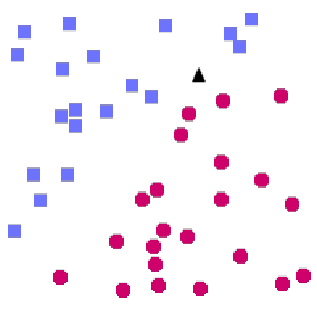
\includegraphics[width=0.5\linewidth]{imagens/image.png}
        \caption{ L’objet à classer (le triangle noir) est-il un rond rouge ou bien un carré bleu ?}
        \label{fig:svm_placeholder_1}
    \end{figure}
\end{frame}

\begin{frame}{Support Vector Machines (SVM)}
    \begin{figure}
        \centering
        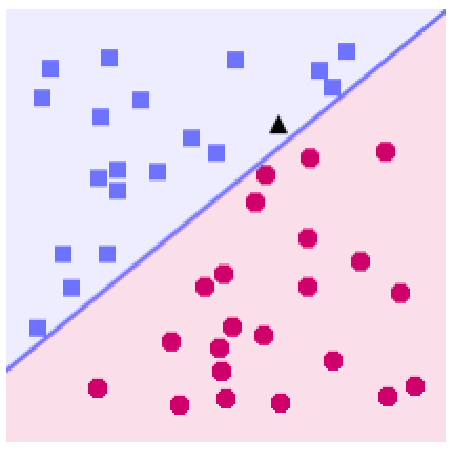
\includegraphics[width=0.5\linewidth]{imagens/image2.png}
        \caption{ Notre SVM, muni des donn’ees d’entraînement (les carr’es bleus et les ronds rouges d’ejà indiqu’es comme tels par l’utilisateur), a tranch’e : le triangle noir est en fait un carre bleu}
        \label{fig:svm_placeholder_2}
    \end{figure}
\end{frame}


% ─── Slide 2 : Formalisme ─────────────────────────────────────────────────────
\begin{frame}{Formalisme des SVM}
    \small
    Pour $x \in \mathbb{R}^n$, le SVM cherche un \textbf{hyperplan affine} :
    \[
    h(x) = \mathbf{w}^\top x + b
    \]
    \begin{itemize}\scriptsize
        \item $\mathbf{w}$ : vecteur de poids \quad $b$ : biais
        \item Classification : $y = +1$ si $h(x) \geq 0$, $\quad y = -1$ sinon
    \end{itemize}
    \vspace{7pt}
    \textbf{Contraintes d'apprentissage}{\scriptsize
    \[
    y_i\,(\langle \mathbf{w}, x_i \rangle + b) \geq 1 \quad \forall i
    \]}
    \vspace{7pt}
    \textbf{Objectif : maximiser la marge}{\scriptsize
    \[
    \text{Marge} = \frac{2}{\|\mathbf{w}\|} \quad \Rightarrow \quad \text{minimiser } \|\mathbf{w}\|
    \]}
\end{frame}

% ─── Slide 3 : Maximisation de la marge ───────────────────────────────────────
\begin{frame}{Maximisation de la marge}
    \small
    \begin{columns}[T]
    \begin{column}{0.55\textwidth}
    \begin{itemize}\scriptsize
        \item $H$ : hyperplan séparateur
        \item $H^+$ : hyperplan longeant les positifs
        \item $H^-$ : hyperplan longeant les négatifs
        \item La \textbf{marge} = distance entre $H^+$ et $H^-$
    \end{itemize}
    \vspace{0.3cm}
    \begin{alertblock}{Résultat clé}\scriptsize
    \[
    \text{Largeur de la marge} = \frac{2}{\|\mathbf{w}\|}
    \]
    $\Rightarrow$ maximiser la marge $=$ minimiser $\|\mathbf{w}\|$
    \end{alertblock}
    \end{column}
    \begin{column}{0.45\textwidth}
    \begin{block}{Distance point-hyperplan}\scriptsize
    \[
    d = \frac{|\mathbf{w}^\top x_k + b|}{\|\mathbf{w}\|}
    \]
    Les \textbf{vecteurs de support} sont les points les plus proches de $H$.
    \end{block}
    \end{column}
    \end{columns}
\end{frame}

\begin{frame}{Maximisation de la marge}
    \begin{figure}
        \centering
        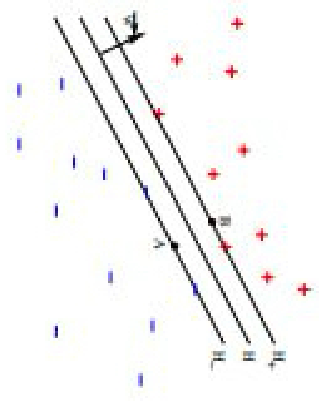
\includegraphics[width=0.4\linewidth]{imagens/Capture d’écran du 2026-01-21 14-11-33.png}
        \caption{Schéma illustratif : groupe H+ et H-}
        \label{fig:svm_placeholder_3}
    \end{figure}
\end{frame}

% ─── Slide 9 : Formulation Lagrangienne ───────────────────────────────────────
\begin{frame}{Formulation Lagrangienne des SVM}
    \small
    \textbf{Problème primal :} minimiser $\frac{1}{2}\|\mathbf{w}\|^2$ sous contraintes $y_i(\mathbf{w}^\top x_i + b) \geq 1$

    \vspace{6pt}
    On introduit les \textbf{multiplicateurs de Lagrange} $\alpha_i \geq 0$ :
    \[
    \mathcal{L}(\mathbf{w}, b, \alpha) = \frac{1}{2}\|\mathbf{w}\|^2 - \sum_{i=1}^{n} \alpha_i \left[ y_i(\mathbf{w}^\top x_i + b) - 1 \right]
    \]

    \begin{columns}[T]
    \begin{column}{0.5\textwidth}
        \textbf{Conditions KKT :}\scriptsize
        \[
        \mathbf{w} = \sum_{i} \alpha_i y_i x_i, \quad \sum_{i} \alpha_i y_i = 0
        \]
        $\Rightarrow$ \textbf{Problème dual} en $\alpha$ uniquement
    \end{column}
    \begin{column}{0.5\textwidth}
        \begin{alertblock}{Propriété clé}\scriptsize
            Seuls les points avec $\alpha_i > 0$ contribuent à $\mathbf{w}$ : ce sont les \textbf{vecteurs de support}.\\[3pt]
            La fonction de décision devient :
            \[
            h(x) = \sum_{i} \alpha_i y_i K(x_i, x) + b
            \]
        \end{alertblock}
    \end{column}
    \end{columns}
\end{frame}

% ─── Slide 4 : SVM non linéaires ──────────────────────────────────────────────
\begin{frame}{SVM non linéaires : Plongée en dimension supérieure}
    \small
    \textbf{Problème :} Certaines données \textbf{ne sont pas linéairement séparables} dans l'espace d'origine (ex: cercles concentriques, problème XOR).
    
    \vspace{7pt}
    \textbf{Solution :} Projeter les données dans un espace de \textbf{dimension supérieure} $E'$ via une fonction $\phi$ :
    \[
    \phi : E \rightarrow E', \quad x \mapsto \phi(x)
    \]
    
    \begin{columns}[T]
    \begin{column}{0.5\textwidth}
    \begin{itemize}\scriptsize
        \item Dans $E'$, les données deviennent linéairement séparables
        \item Le SVM trouve un hyperplan dans $E'$
        \item Ce plan correspond à une \textbf{frontière non linéaire} dans $E$
    \end{itemize}
    \end{column}
    \begin{column}{0.5\textwidth}
    \begin{alertblock}{Problème pratique}\scriptsize
    Plus la dimension de $E'$ est grande, plus les calculs sont \textbf{coûteux}.\\
    $\Rightarrow$ Le \textbf{Kernel Trick} résout ce problème !
    \end{alertblock}
    \end{column}
    \end{columns}
\end{frame}

\begin{frame}{SVM non linéaires : Plongée en dimension supérieure}
    \begin{figure}
        \centering
        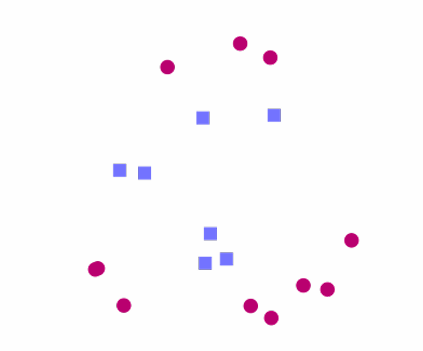
\includegraphics[width=0.5\linewidth]{imagens/donnees_non_lineaires.png}
        \caption{Données d’entraînement non linéairement séparables}
        \label{fig:svm_placeholder_4}
    \end{figure}
\end{frame}

\begin{frame}{SVM non linéaires : Plongée en dimension supérieure}
    \begin{figure}
        \centering
        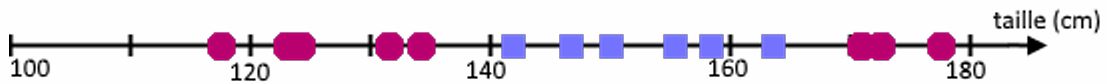
\includegraphics[width=\linewidth]{imagens/donnees_droite.png}
        \caption{Illustration : données sur une droite}
        \label{fig:svm_placeholder_5}
    \end{figure}
\end{frame}

\begin{frame}{SVM non linéaires : Plongée en dimension supérieure}
    \begin{figure}
        \centering
        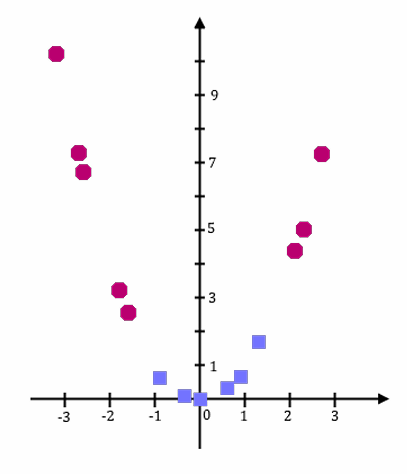
\includegraphics[width=0.5\linewidth]{imagens/projection_r2.png}
        \caption{Données d’entraînement après projection dans l’espace R2}
        \label{fig:svm_placeholder_6}
    \end{figure}
\end{frame}

% ─── Slide 5 : Kernel Trick ───────────────────────────────────────────────────
\begin{frame}{L'Astuce du Noyau (Kernel Trick)}
    \small
    \textbf{Idée centrale : } 
    Les algorithmes n'ont besoin que des \textbf{produits scalaires} $\phi(x_i)^\top \phi(x_j)$.\\
    On définit une \textbf{fonction noyau} : $K(x, x') = \phi(x)^\top \phi(x')$
    
    \vspace{8pt}
    \begin{columns}[T]
    \begin{column}{0.5\textwidth}
    \textbf{Principaux noyaux :}
    \begin{itemize}\scriptsize
        \item \textbf{Polynomial :} $K = (\alpha\, x^\top x' + \lambda)^d$
        \item \textbf{Gaussien (RBF) :} $K = \exp\!\left(-\frac{\|x-x'\|^2}{2\sigma^2}\right)$
        \item \textbf{Laplacien :} $K = \exp\!\left(-\frac{\|x-x'\|}{\sigma}\right)$
        \item \textbf{Rationnel quadratique}
    \end{itemize}
    \end{column}
    \begin{column}{0.5\textwidth}
    \begin{alertblock}{Avantage}\scriptsize
    Calcul en $\mathcal{O}(n)$ au lieu de $\mathcal{O}(n^2)$ pour le produit dans $E'$.\\[4pt]
    Pas besoin de connaître $E'$ ni $\phi$ explicitement !
    \end{alertblock}
    \end{column}
    \end{columns}
\end{frame}

% ─── Slide 7 : Types de noyaux ────────────────────────────────────────────────
\begin{frame}{Types de noyaux}
    \small
    \begin{tabular}{|l|l|l|}
        \hline
        \textbf{Noyau} & \textbf{Formule} & \textbf{Usage} \\
        \hline
        Linéaire & $x^\top x'$ & Données séparables \\
        \hline
        Polynomial & $(\alpha\, x^\top x' + \lambda)^d$ & Écriture, NLP \\
        \hline
        Gaussien (RBF) & $\exp\!\left(-\frac{\|x-x'\|^2}{2\sigma^2}\right)$ & Usage général \\
        \hline
        Laplacien & $\exp\!\left(-\frac{\|x-x'\|}{\sigma}\right)$ & Bio-informatique \\
        \hline
        Rat. Quadratique & $1 - \frac{\|x-x'\|^2}{\|x-x'\|^2 + \sigma}$ & Recommandation \\
        \hline
    \end{tabular}

    \vspace{6pt}
    \begin{alertblock}{Condition de Mercer}\scriptsize
        Une fonction $K$ est un noyau valide si et seulement si elle est \textbf{continue, symétrique et semi-définie positive} :
        $\displaystyle\sum_{i,j} c_i c_j K(x_i, x_j) \geq 0$
    \end{alertblock}
\end{frame}

% ─── Slide 8 : Hyperparamètres ────────────────────────────────────────────────
\begin{frame}{Hyperparamètres clés des SVM}
    \small
    \begin{columns}[T]
    \begin{column}{0.5\textwidth}
        \textbf{Paramètre $C$ (régularisation) \\}{\scriptsize
            Contrôle le \textbf{compromis biais-variance} :
            \begin{itemize}
                \item $C$ grand $\Rightarrow$ marge étroite, peu d'erreurs tolérées $\Rightarrow$ surapprentissage
                \item $C$ petit $\Rightarrow$ marge large, plus d'erreurs tolérées $\Rightarrow$ sous-apprentissage
            \end{itemize}}
            
        \vspace{4pt}
        \textbf{Paramètre $\sigma$ / $\gamma$ (noyau RBF) \\}{\scriptsize
            Contrôle la \textbf{portée d'influence} de chaque point :
            \begin{itemize}
                \item $\sigma$ petit $\Rightarrow$ frontière très locale
                \item $\sigma$ grand $\Rightarrow$ frontière lissée
            \end{itemize}}
    \end{column}
    \begin{column}{0.5\textwidth}
        \textbf{Paramètre $d$ (noyau polynomial) \\}{\scriptsize
            Degré du polynôme :\\
            plus $d$ est grand, plus la frontière est complexe.}
            
        \vspace{4pt}
        \begin{alertblock}{Stratégie de réglage}\scriptsize
            Utiliser la \textbf{validation croisée} (grid search) pour trouver la combinaison $(C, \sigma)$ optimale.\\[3pt]
            Mauvais choix $\Rightarrow$ dégradation sévère des performances.
        \end{alertblock}
    \end{column}
    \end{columns}
\end{frame}

% ─── Slide 6 : Avantages, Limites & Conclusion ────────────────────────────────
\begin{frame}{Conclusion SVM}
    \small
    \begin{columns}[T]
    \begin{column}{0.5\textwidth}
    \textbf{Avantages}\scriptsize
    \begin{itemize}
        \item Efficace en \textbf{grande dimension}
        \item Robuste au \textbf{surapprentissage}
        \item Fonctionne avec peu de données
        \item Frontières complexes via noyaux
        \item Optimum \textbf{global} garanti
    \end{itemize}
    \end{column}
    \begin{column}{0.5\textwidth}
    \textbf{Limites}\scriptsize
    \begin{itemize}
        \item Sensible au choix des \textbf{hyperparamètres} ($C$, $\sigma$)
        \item Coûteux pour de \textbf{grands jeux} de données
        \item Choix du noyau non trivial
        \item Moins interprétable que les arbres
    \end{itemize}
    \end{column}
    \end{columns}
    
    \vspace{0.2cm}
    \begin{alertblock}{Message clé}\scriptsize
    Les SVM cherchent l'\textbf{hyperplan à marge maximale}. Pour les données non linéaires, le \textbf{Kernel Trick} permet de travailler implicitement dans un espace de grande dimension, sans en calculer explicitement les coordonnées.
    \end{alertblock}
\end{frame}

\section{Bagging vs Boosting}
% ─────────────────────────────────────────────
% IMAGE SLIDE : Bagging vs Boosting
\begin{frame}{Concepts clés : Bagging vs Boosting}
\begin{figure}
    \centering
    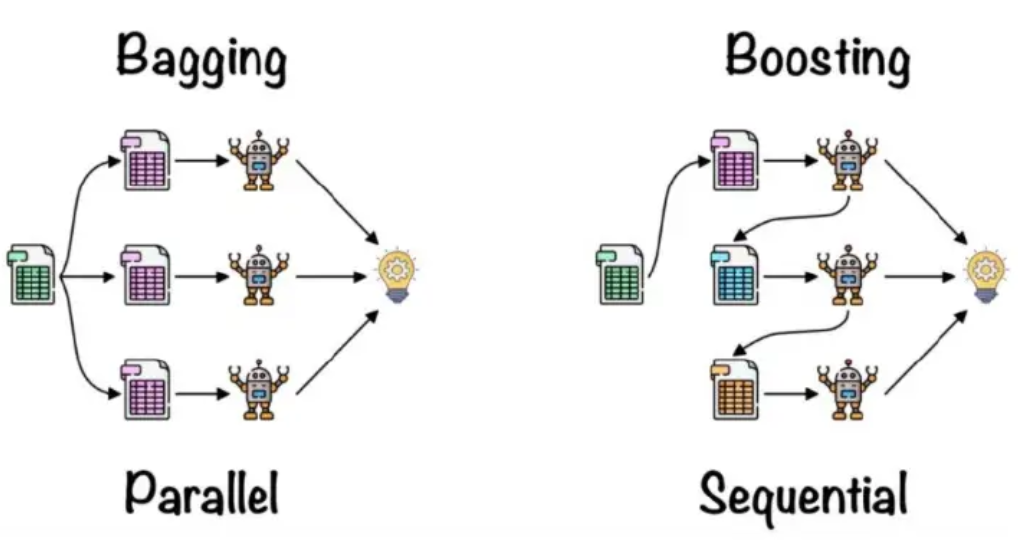
\includegraphics[width=0.95\linewidth]{bagging vs boosting.png}
    \caption{Bagging (parallèle, réduit la variance) vs Boosting (séquentiel, réduit le biais).}
\end{figure}
\end{frame}

\section{Random Forests}
% ─────────────────────────────────────────────
\begin{frame}{Introduction aux Random Forests}
\begin{itemize}
    \item Les arbres de décision simples sont sujets au \textbf{surapprentissage (overfitting)}.
    
    \medskip
    \item Les \textbf{Random Forests} combinent plusieurs arbres pour un modèle plus \textbf{robuste et précis}.
    
    \medskip
    \item Principe clé : la \textit{sagesse des foules} — agréger les prédictions de nombreux arbres entraînés sur des sous-échantillons différents.
    
    \medskip
    \item Contrairement aux SVM et à XGBoost, les Random Forests construisent des arbres \textbf{indépendants et parallèles}.
\end{itemize}
\end{frame}

% ─────────────────────────────────────────────
\begin{frame}{Fonctionnement du Random Forest}
\begin{figure}
    \centering
    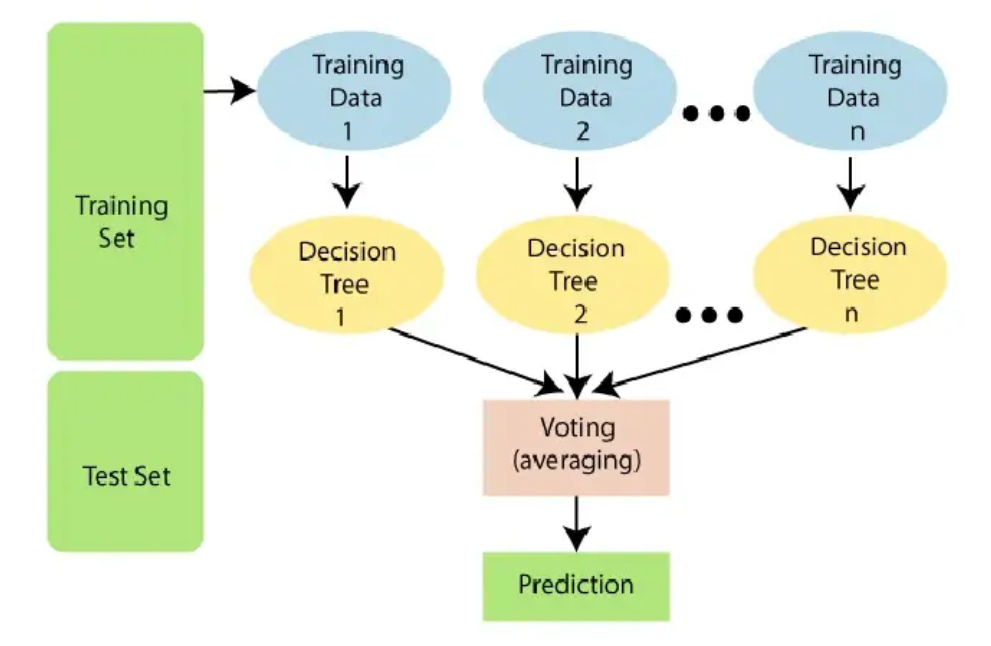
\includegraphics[width=0.9\linewidth]{fonctionnement.png}
    \caption{Principe de fonctionnement du Random Forest}
\end{figure}
\end{frame}


% ─────────────────────────────────────────────
% IMAGE SLIDE : Decision Tree

\begin{frame}{Rappel : Arbres de décision}
\begin{itemize}
    \item Un \textbf{arbre de décision} est un modèle hiérarchique basé sur une succession de questions binaires (oui/non).
    \item Il est composé de :
    \begin{itemize}
        \item \textbf{Nœuds internes} : décisions sur les variables d'entrée ;
        \item \textbf{Branches} : résultats possibles des décisions ;
        \item \textbf{Feuilles} : prédictions finales.
    \end{itemize}
    \item Exemple : « Âge > 30 ? », puis « Revenu > 50\,000 ? » pour prédire un achat.
\end{itemize}
\end{frame}
\begin{frame}{Rappel visuel : Arbre de décision}
\begin{figure}
    \centering
    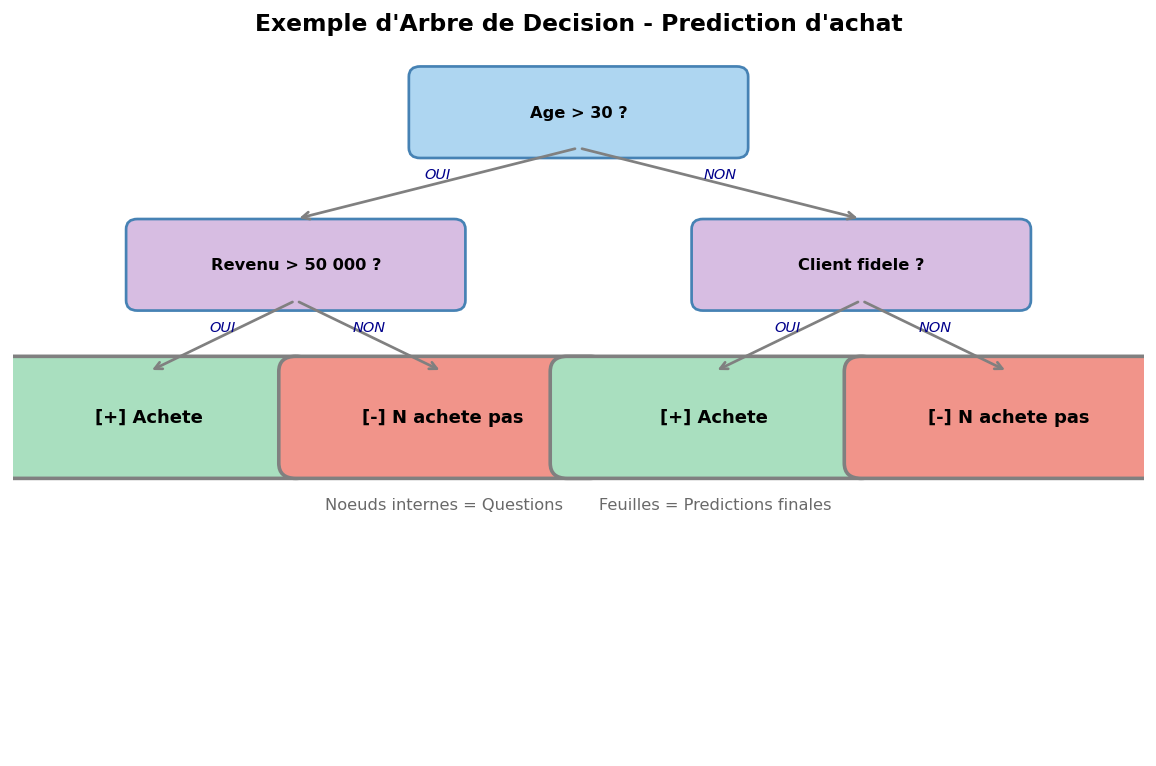
\includegraphics[width=0.8\textwidth]{decision_tree.png}
    \caption{Exemple d'arbre de décision pour la prédiction d'un achat.}
\end{figure}
\end{frame}

\begin{frame}{Construction récursive et surapprentissage}
\begin{itemize}
    \item L'arbre se construit de manière \textbf{récursive} en choisissant à chaque étape la meilleure division.
    \item Sans contraintes, l'arbre peut \textbf{surapprendre} :
    \begin{itemize}
        \item Excellente performance sur les données d'entraînement ;
        \item Mauvaise généralisation sur de nouvelles données.
    \end{itemize}
    \item Les arbres ont \textbf{faible biais} mais \textbf{forte variance} → motivation des Random Forests.
\end{itemize}
\end{frame}

% ─────────────────────────────────────────────
\begin{frame}{Algorithme des Random Forests}
\begin{itemize}
    \item Deux sources principales de hasard :
    \begin{itemize}
        \item L'\textbf{échantillonnage bootstrap} des données ;
        \item La \textbf{sélection aléatoire des caractéristiques}.
    \end{itemize}
    \item Ces mécanismes permettent de construire un ensemble d'arbres \textbf{diversifiés et moins corrélés}.
\end{itemize}
\end{frame}

\begin{frame}{Étape 1 : Échantillonnage Bootstrap}
\begin{itemize}
    \item Pour chaque arbre, on génère un échantillon aléatoire \textbf{avec remise}.
    \item Certaines observations peuvent apparaître plusieurs fois, d'autres peuvent être absentes.
    \item En moyenne, chaque échantillon contient environ \textbf{63,2\%} d'observations uniques.
    \item Cela crée des jeux de données légèrement différents pour entraîner chaque arbre.
\end{itemize}
\end{frame}

\begin{frame}{Étape 2 : Sélection aléatoire des caractéristiques}
\begin{itemize}
    \item À chaque nœud, on sélectionne aléatoirement un sous-ensemble de caractéristiques ($m < p$).
    \item La meilleure division est choisie \textbf{uniquement parmi ces caractéristiques}.
    \item Objectif : réduire la corrélation entre les arbres et augmenter la \textbf{diversité} du modèle.
\end{itemize}
\end{frame}

\begin{frame}{Étapes 3 et 4 : Croissance et Agrégation}
\begin{itemize}
    \item \textbf{Croissance des arbres} :
    \begin{itemize}
        \item Chaque arbre est développé jusqu'à sa profondeur maximale (sans élagage).
    \end{itemize}
    
    \medskip
    \item \textbf{Agrégation des prédictions} :
    \begin{itemize}
        \item Classification : \textbf{vote majoritaire} des arbres ;
        \item Régression : \textbf{moyenne} des prédictions.
    \end{itemize}
\end{itemize}
\end{frame}

\begin{frame}{Hyperparamètre clé : Nombre d'arbres}
\begin{itemize}
    \item \textbf{n\_estimators (ntree)} : nombre d'arbres dans la forêt.
    \item Valeurs typiques : 100 à 1000 arbres.
    \item Effets :
    \begin{itemize}
        \item Plus d'arbres $\rightarrow$ variance réduite et prédictions plus stables ;
        \item Temps de calcul plus élevé.
    \end{itemize}
    \item Les gains deviennent faibles après un certain seuil (plateau de performance).
    \item Contrairement au boosting, ajouter des arbres ne provoque généralement \textbf{pas de surapprentissage}.
\end{itemize}
\end{frame}

\begin{frame}{Hyperparamètre clé : max\_features}
\begin{itemize}
    \item Contrôle le nombre de caractéristiques testées à chaque division.
    \item Valeurs par défaut :
    \begin{itemize}
        \item Classification : $\sqrt{p}$
        \item Régression : $p/3$
    \end{itemize}
    \item Effets :
    \begin{itemize}
        \item Valeurs faibles $\rightarrow$ arbres plus diversifiés mais plus faibles ;
        \item Valeurs élevées $\rightarrow$ arbres plus puissants mais plus corrélés.
    \end{itemize}
    \item C'est l'hyperparamètre le \textbf{plus important} à ajuster.
\end{itemize}
\end{frame}

\begin{frame}{Autres hyperparamètres et stratégie d'ajustement}
\begin{itemize}
    \item \textbf{Profondeur des arbres} :
    \begin{itemize}
        \item max\_depth, min\_samples\_split, min\_samples\_leaf
    \end{itemize}
    
    \medskip
    \item \textbf{Taille bootstrap (max\_samples)} :
    \begin{itemize}
        \item Fraction des données utilisée pour chaque arbre.
    \end{itemize}
    
    \medskip
    \item \textbf{Stratégie pratique} :
    \begin{enumerate}
        \item Commencer avec les paramètres par défaut ;
        \item Ajuster d'abord n\_estimators ;
        \item Ajuster ensuite max\_features (le plus influent) ;
        \item Utiliser l'erreur OOB pour une évaluation rapide.
    \end{enumerate}
\end{itemize}
\end{frame}

% ─────────────────────────────────────────────
% IMAGE SLIDE : OOB
\begin{frame}{Estimation de l'erreur Out-of-Bag (OOB) — Illustration}
\begin{figure}
    \centering
    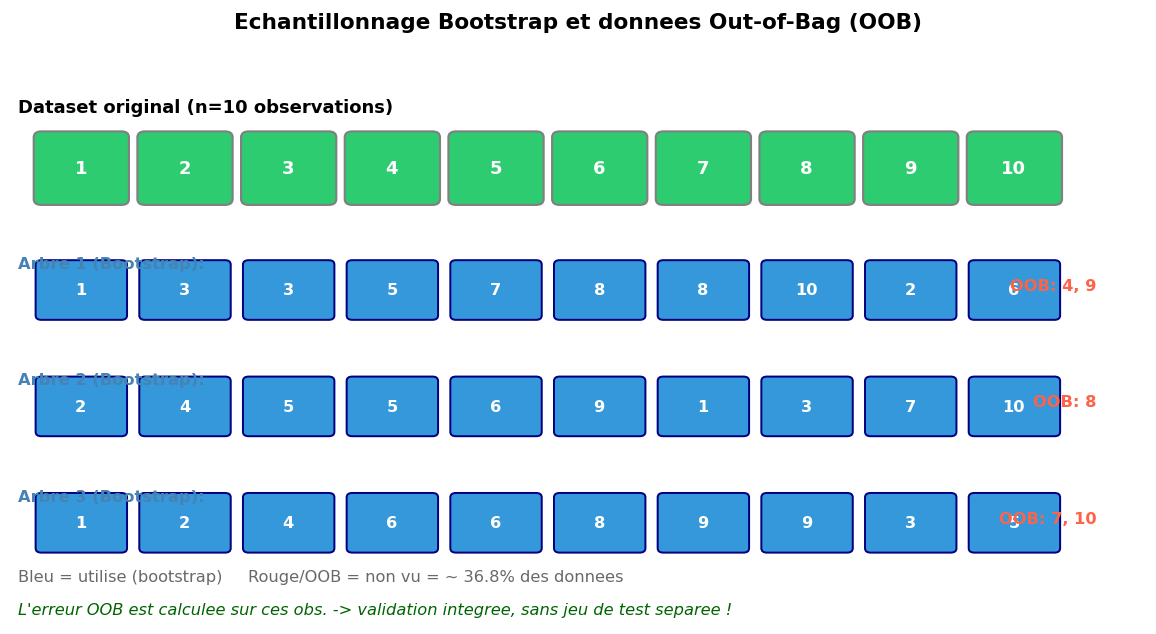
\includegraphics[width=0.92\linewidth]{imagens/oob_bootstrap.png}
    \caption{Schéma du mécanisme bootstrap et des données OOB par arbre.}
\end{figure}
\end{frame}

\begin{frame}{Fonctionnement de l'erreur Out-of-Bag (OOB)}
\begin{itemize}
    \item Lors du bootstrap, environ \textbf{36,8\%} des observations ne sont pas utilisées pour entraîner un arbre donné : ce sont les \textbf{échantillons Out-of-Bag (OOB)}.
    
    \medskip
    \item Pour chaque observation :
    \begin{enumerate}
        \item Identifier les arbres qui ne l'ont pas vue (arbres OOB).
        \item Faire la prédiction uniquement avec ces arbres.
        \item Comparer la prédiction à la vraie valeur.
    \end{enumerate}
    
    \medskip
    \item L'erreur OOB = moyenne des erreurs sur toutes les observations.
    
    \medskip
    \textbf{Avantage :} validation intégrée sans jeu de test séparé.
\end{itemize}
\end{frame}

\begin{frame}{Avantages et limites de l'erreur OOB}
\textbf{Avantages :}
\begin{itemize}
    \item Estimation \textbf{non biaisée} de l'erreur de généralisation
    \item Aucun coût d'entraînement supplémentaire
    \item Permet de choisir le nombre d'arbres optimal
\end{itemize}

\medskip
\textbf{Limites :}
\begin{itemize}
    \item Peut être légèrement \textbf{optimiste} comparée à un test indépendant
    \item Moins fiable sur de \textbf{petits jeux de données}
\end{itemize}

\medskip
\textbf{Formule clé :}
\[
P(\text{non sélectionnée}) = \left(1 - \frac{1}{n}\right)^n \rightarrow \frac{1}{e} \approx 0{,}368
\]
\end{frame}

% ─────────────────────────────────────────────
% IMAGE SLIDE : Feature Importance
\begin{frame}{Importance des variables — Illustration}
\begin{figure}
    \centering
    
\includegraphics[width=0.90\linewidth]{feature_importance.png}
    \caption{Importance MDI (Gini) des variables pour la prédiction du prix des maisons.}
\end{figure}
\end{frame}

\begin{frame}{Importance des variables : MDI (Gini Importance)}
\begin{itemize}
    \item La \textbf{Diminution Moyenne de l'Impureté (MDI)} mesure combien une variable réduit l'impureté des nœuds.
    
    \medskip
    \item Calcul : sommer la réduction d'impureté pondérée sur tous les arbres et normaliser.
    
    \medskip
    \item \textbf{Limites :}
    \begin{itemize}
        \item Biais vers les variables à forte cardinalité
        \item Peut surestimer l'importance si les variables sont corrélées
    \end{itemize}
\end{itemize}
\end{frame}

% ─────────────────────────────────────────────
\begin{frame}{Avantages des Random Forests}
\begin{itemize}
    \item Robustesse au surapprentissage
    \item Prétraitement minimal des données
    \item Gestion des valeurs manquantes
    \item Capture naturelle des relations non linéaires
    \item Parallélisation et scalabilité
    \item Validation intégrée (erreur OOB)
    \item Importance des variables interprétable
    \item Bonnes performances avec paramètres par défaut
    \item Polyvalence (classification, régression, etc.)
\end{itemize}
\end{frame}

\begin{frame}{Limitations des Random Forests}
\begin{itemize}
    \item Difficulté d'interprétation
    \item Besoins élevés en mémoire
    \item Vitesse de prédiction plus lente
    \item Moins performant sur données hautement dimensionnelles
    \item Pas d'extrapolation en régression
    \item Importance des variables biaisée (MDI)
    \item Pas toujours le meilleur choix face au boosting ou deep learning
\end{itemize}
\end{frame}

\begin{frame}{Conclusion Random Forest}
\begin{itemize}
    \item Les Random Forests sont des modèles puissants et polyvalents basés sur le \textbf{bagging}
    \item Robustesse au surapprentissage et gestion des relations non linéaires
    \item Validation intégrée via l'\textbf{erreur Out-of-Bag (OOB)}
    \item Adaptées à la classification et à la régression
    \item Limites : interprétation difficile et coût mémoire élevé
    \item XGBoost adopte une approche \textbf{boosting} avec construction séquentielle des arbres
\end{itemize}
\end{frame}

\section{XGBoost}

% ─────────────────────────────────────────────
\begin{frame}{Introduction à XGBoost}
\begin{itemize}
    \item \textbf{XGBoost} (eXtreme Gradient Boosting) : algorithme avancé de gradient boosting
    
    \item Introduit par Chen \& Guestrin (2016)
    
    \item Optimisé, scalable et performant pour classification et régression
    
    \item Large succès en compétitions Kaggle et applications industrielles
    \item Utilise le \textbf{boosting} (construction séquentielle) pour réduire le biais
    \item Alternative performante aux méthodes basées sur le bagging (Random Forest)
\end{itemize}
\end{frame}

% ─────────────────────────────────────────────
% IMAGE : Principe du Gradient Boosting — résidus

\begin{frame}{Caractéristiques et innovations de XGBoost}
\textbf{Points clés qui distinguent XGBoost du Gradient Boosting classique :}
\begin{itemize}
    \item \textbf{Régularisation} intégrée 
    \item Conception d'\textbf{un arbre de régression unique} optimisé
    \item \textbf{Algorithme glouton approximatif} pour le choix des coupures
    \item \textbf{Esquisse de quantiles pondérés} (weighted quantile sketch)
    \item Intégration de la parcimonie des données (\textbf{sparsity-aware split finding})
    \item \textbf{Apprentissage parallèle} au niveau des nœuds
    \item \textbf{Accès optimisé au cache} du processeur (cache-aware access)
    \item \textbf{Calculs hors mémoire par blocs} (out-of-core computation)
\end{itemize}
\end{frame}

\begin{frame}{Principe du Gradient Boosting}
\begin{itemize}
    \item Apprentissage \textbf{itératif et séquentiel}
    \item Chaque nouvel arbre apprend les \textbf{erreurs résiduelles} du modèle précédent
    \item Construction progressive du modèle global
    \item Interprétation : descente de gradient dans l'espace des fonctions
    \item Objectif : minimisation incrémentale de la \textbf{fonction de perte}
\end{itemize}
\end{frame}
\begin{frame}{Principe du Gradient Boosting — Illustration}
\begin{figure}
    \centering
    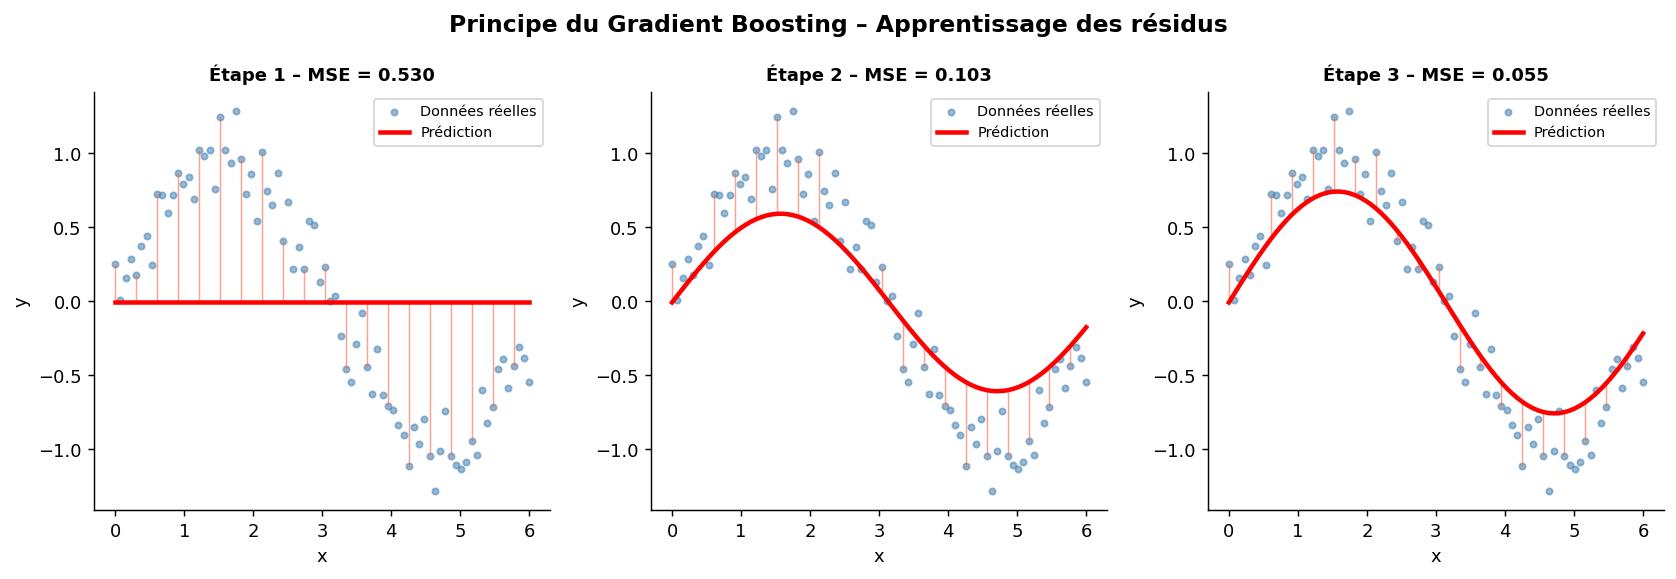
\includegraphics[width=0.97\linewidth]{imagens/gradient_boosting_residuals.png}
    \caption{Chaque arbre réduit progressivement les résidus du modèle précédent.}
\end{figure}
\end{frame}
% ─────────────────────────────────────────────
% IMAGE : Construction séquentielle XGBoost
\begin{frame}{XGBoost : Construction séquentielle}
\begin{figure}
    \centering
    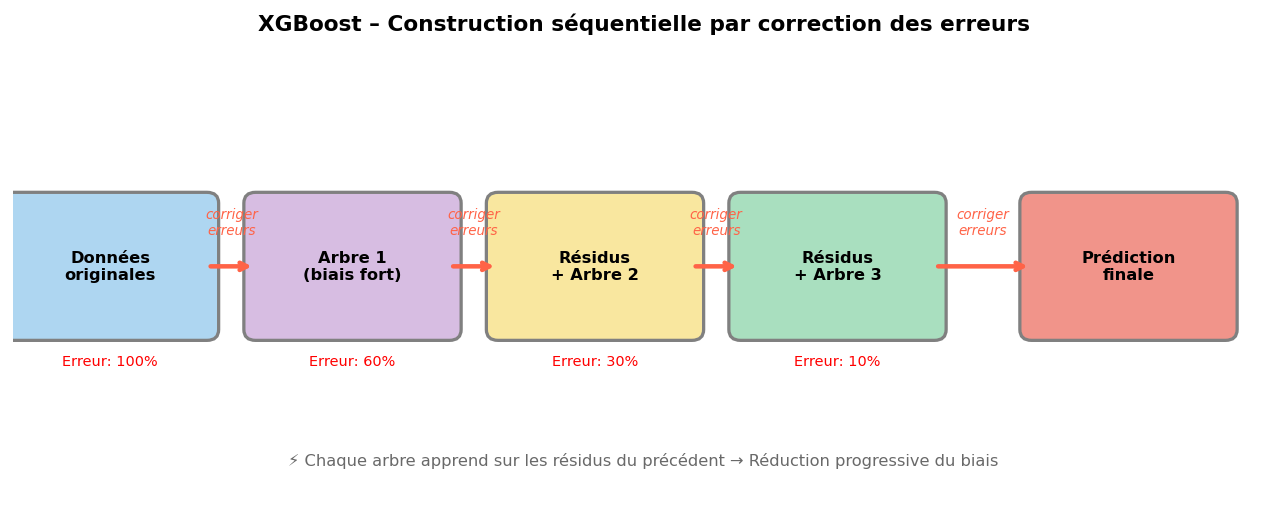
\includegraphics[width=0.95\linewidth]{imagens/xgboost_sequential.png}
    \caption{XGBoost corrige progressivement les erreurs des modèles précédents.}
\end{figure}
\end{frame}

\begin{frame}{XGBoost pour la Régression : Initialisation}
    \begin{columns}[T]
        \begin{column}{0.42\textwidth}
            \textbf{Jeu de données (Médicaments) :}
            
            \begin{table}
                \centering
                \scriptsize
                \begin{tabular}{|c|c|}
                    \hline
                    \textbf{Dosage (mg)} & \textbf{Efficacité} \\
                    \hline
                    10 & -10 \\
                    20 & 7 \\
                    25 & 8 \\
                    35 & -7 \\
                    \hline
                \end{tabular}
            \end{table}
            
            \begin{block}{Prédiction initiale $f_0(x)$}
                \scriptsize
                Valeur par défaut : \textbf{0.5}.
                
                \textbf{Pourquoi 0.5 ?} \\
                Dans XGBoost, le score de base (\texttt{base\_score}) est initialisé à 0.5 par défaut, un héritage de la probabilité. En régression, ce "décalage" n'est pas pénalisant : les arbres de gradient vont très vite corriger cette valeur initiale via l'apprentissage itératif des résidus.
            \end{block}
        \end{column}
        
        \begin{column}{0.58\textwidth}
            \begin{center}
            \begin{tikzpicture}[x=0.11cm, y=0.25cm, every node/.style={scale=0.75}]
                % Axes
                \draw[->, thick, -latex] (0,-11) -- (0,11) node[above] {Efficacité ($y$)};
                \draw[->, thick, -latex] (0,0) -- (45,0) node[right] {Dosage};
                
                % Ticks sur l'axe Y
                \foreach \y in {-10, -9,-8,-7, -5, -3, -1, 1, 3, 5, 7, 8, 9} {
                    \draw (2pt,\y) -- (-2pt,\y) node[left] {\y};
                }
                
                % Ticks sur l'axe X
                \foreach \x in {10, 20, 25, 35} {
                    \draw (\x, 2pt) -- (\x, -2pt) node[below=2pt] {\x};
                }
                
                % Points de données
                \fill[blue] (10,-10) circle (3pt);
                \fill[blue] (20,7) circle (3pt);
                \fill[blue] (25,8) circle (3pt);
                \fill[blue] (35,-7) circle (3pt);
                
                % Ligne de prédiction initiale 0.5
                \draw[thick, red] (0, 0.5) -- (42, 0.5) node[right] {$f_0(x) = 0.5$};
                
                % Projection des points vers l'axe x
                \draw[dashed, blue!50] (10,0) -- (10,-10);
                \draw[dashed, blue!50] (20,0) -- (20,7);
                \draw[dashed, blue!50] (25,0) -- (25,8);
                \draw[dashed, blue!50] (35,0) -- (35,-7);

            \end{tikzpicture}
            \end{center}
        \end{column}
    \end{columns}
\end{frame}

% Frame 2 : Résidus et Formules
\begin{frame}{XGBoost pour la Régression : Résidus et Formules}
    \begin{columns}[T]
        \begin{column}{0.4\textwidth}
            \textbf{Calcul des Résidus ($r_i$) :} \\
            $r_i = y_i - f_0(x_i)$ \\
            \scriptsize (\textit{Efficacité réelle - prédiction})
            \vspace{0.1cm}
            
            \begin{table}
                \centering
                \scriptsize
                \begin{tabular}{|c|c|c|}
                    \hline
                    \textbf{Dosage} & \textbf{Effic.} & \textbf{Résidu ($r_i$)} \\
                    \hline
                    10 & -10 & \textbf{-10.5} \\
                    20 & 7 & \textbf{6.5} \\
                    25 & 8 & \textbf{7.5} \\
                    35 & -7 & \textbf{-7.5} \\
                    \hline
                \end{tabular}
            \end{table}
            
            \vspace{0.2cm}
            \scriptsize
            \textit{Exemple pour dosage 10 :} \\
            $r_1 = -10 - 0.5 = -10.5$
        \end{column}
        
        \begin{column}{0.6\textwidth}
            \begin{block}{Métriques de construction}
                \scriptsize
                \textbf{1. Similarity Score (SS) :}
                $ SS = \frac{(\sum \text{Résidus})^2}{\text{Nb. Résidus} + \lambda} $ \\
                \textit{Évalue la pureté du nœud.}
                
                \textbf{2. Gain :} 
                $ Gain = SS_{gauche} + SS_{droit} - SS_{racine} - \gamma $ \\
                \textit{Mesure l'amélioration apportée par l'embranchement.}
                
                \textbf{3. Hyperparamètres de Régularisation :}
                \begin{itemize}
                    \setlength\itemsep{0em}
                    \item $\lambda$ (Lambda) : Régularisation L2. Diminue l'influence des observations individuelles.
                    \item $\gamma$ (Gamma) : Seuil minimal de Gain requis pour diviser.
                \end{itemize}
            \end{block}
         
            \scriptsize
            \textbf{Score de la Racine} (avec $\lambda=0$) : \\
            Somme des résidus = -4. Nombre = 4. \\
            $\rightarrow SS_{racine} = \frac{(-4)^2}{4+0} = \frac{16}{4} = 4$.
        \end{column}
    \end{columns}
\end{frame}

% Frame 3 : Splits 1 et 2
\begin{frame}{XGBoost : Évaluation des Splits (Arbre 1)}
    \vspace{-0.2cm}
    \textit{\small On évalue les moyennes entre dosages consécutifs : 15, 22.5, 30. ($\lambda=0, \gamma=0$)}
    
    \begin{columns}[T]
        % SPLIT 1
        \begin{column}{0.5\textwidth}
            \begin{block}{Split 1 : Dosage < 15}
                \centering
                \begin{tikzpicture}[every node/.style={scale=0.6}, level/.style={sibling distance=2.5cm, level distance=1.1cm}]
                    \node[draw, rectangle, fill=gray!20, text width=2.5cm, align=center] {Racine \\ $SS = 4$}
                        child {node[draw, rectangle, fill=blue!10, text width=2.4cm, align=center] {Dosage < 15 \\ $r=\{-10.5\}$ \\ $SS = 110.25$}}
                        child {node[draw, rectangle, fill=red!10, text width=2.9cm, align=center] {Dosage $\geq$ 15 \\ $r=\{6.5, 7.5, -7.5\}$ \\ $SS = 14.08$}};
                \end{tikzpicture}
                \vspace{0.1cm}
                
                \footnotesize \textbf{Gain} $= 110.25 + 14.08 - 4 = \textbf{120.33}$
                
                \vspace{0.1cm}
                \begin{tikzpicture}[x=0.08cm, y=0.08cm, every node/.style={scale=0.55}]
                    \draw[->, thick, -latex] (0,-11) -- (0,11);
                    \draw[->, thick, -latex] (0,0) -- (45,0);
                    \fill[blue] (10,-10) circle (3pt); \fill[blue] (20,7) circle (3pt);
                    \fill[blue] (25,8) circle (3pt); \fill[blue] (35,-7) circle (3pt);
                    \draw[thick, red] (0, 0.5) -- (42, 0.5);
                    \draw[thick, green!70!black, dashed] (15, -11) -- (15, 11) node[pos=0.9, right] {x=15};
                \end{tikzpicture}
            \end{block}
        \end{column}
        
        % SPLIT 2
        \begin{column}{0.5\textwidth}
            \begin{block}{Split 2 : Dosage < 22.5}
                \centering
                \begin{tikzpicture}[every node/.style={scale=0.6}, level/.style={sibling distance=2.5cm, level distance=1.1cm}]
                    \node[draw, rectangle, fill=gray!20, text width=2.5cm, align=center] {Racine \\ $SS = 4$}
                        child {node[draw, rectangle, fill=blue!10, text width=2.6cm, align=center] {Dosage < 22.5 \\ $r=\{-10.5, 6.5\}$ \\ $SS = 8$}}
                        child {node[draw, rectangle, fill=red!10, text width=2.5cm, align=center] {Dosage $\geq$ 22.5 \\ $r=\{7.5, -7.5\}$ \\ $SS = 0$}};
                \end{tikzpicture}
                \vspace{0.1cm}
                
                \footnotesize \textbf{Gain} $= 8 + 0 - 4 = \textbf{4.00}$
                
                \vspace{0.1cm}
                \begin{tikzpicture}[x=0.08cm, y=0.08cm, every node/.style={scale=0.55}]
                    \draw[->, thick, -latex] (0,-11) -- (0,11);
                    \draw[->, thick, -latex] (0,0) -- (45,0);
                    \fill[blue] (10,-10) circle (3pt); \fill[blue] (20,7) circle (3pt);
                    \fill[blue] (25,8) circle (3pt); \fill[blue] (35,-7) circle (3pt);
                    \draw[thick, red] (0, 0.5) -- (42, 0.5);
                    \draw[thick, green!70!black, dashed] (22.5, -11) -- (22.5, 11) node[pos=0.9, right] {x=22.5};
                \end{tikzpicture}
            \end{block}
        \end{column}
    \end{columns}
\end{frame}

% Frame 4 : Split 3 et Conclusion
\begin{frame}{XGBoost : Split 3 et Conclusion de l'Arbre 1}
    \begin{columns}[T]
        % SPLIT 3
        \begin{column}{0.5\textwidth}
            \begin{block}{Split 3 : Dosage < 30}
                \centering
                \begin{tikzpicture}[every node/.style={scale=0.6}, level/.style={sibling distance=2.8cm, level distance=1.1cm}]
                    \node[draw, rectangle, fill=gray!20, text width=2.5cm, align=center] {Racine \\ $SS = 4$}
                        child {node[draw, rectangle, fill=blue!10, text width=3.3cm, align=center] {Dosage < 30 \\ $r=\{-10.5, 6.5, 7.5\}$ \\ $SS = 4.08$}}
                        child {node[draw, rectangle, fill=red!10, text width=2.0cm, align=center] {Dosage $\geq$ 30 \\ $r=\{-7.5\}$ \\ $SS = 56.25$}};
                \end{tikzpicture}
                \vspace{0.1cm}
                
                \footnotesize \textbf{Gain} $= 4.08 + 56.25 - 4 = \textbf{56.33}$
                
                \vspace{0.1cm}
                \begin{tikzpicture}[x=0.08cm, y=0.08cm, every node/.style={scale=0.55}]
                    \draw[->, thick, -latex] (0,-11) -- (0,11);
                    \draw[->, thick, -latex] (0,0) -- (45,0);
                    \fill[blue] (10,-10) circle (3pt); \fill[blue] (20,7) circle (3pt);
                    \fill[blue] (25,8) circle (3pt); \fill[blue] (35,-7) circle (3pt);
                    \draw[thick, red] (0, 0.5) -- (42, 0.5);
                    \draw[thick, green!70!black, dashed] (30, -11) -- (30, 11) node[pos=0.9, right] {x=30};
                \end{tikzpicture}
            \end{block}
        \end{column}
        
        % VERDICT
        \begin{column}{0.5\textwidth}
            \begin{block}{Comparaison des Splits ($\lambda=0, \gamma=0$)}
                \scriptsize
                \begin{itemize}
                    \setlength\itemsep{0em}
                    \item Gain (Split < 15) : \textbf{120.33}
                    \item Gain (< 22.5) : 4.00 \quad | \quad Gain (< 30) : 56.33
                \end{itemize}
            \end{block}
            
            \begin{block}{Verdict de l'algorithme}
                \scriptsize
                L'approche gloutonne (Greedy Algorithm) sélectionne le split \textbf{maximisant le Gain}.
                
                $\Rightarrow$ On isole la valeur très négative en coupant à \textbf{Dosage < 15}.
                
                \vspace{0.1cm}
                \tiny \textit{Le processus se répète ensuite de façon récursive sur les nœuds enfants.}
            \end{block}
        \end{column}
    \end{columns}
\end{frame}

% Frame 5 : Poursuite de l'arbre
\begin{frame}{XGBoost : Poursuite de la construction (Nœud Droit)}
    \vspace{-0.2cm}
    \textit{\small Le nœud de droite (Dosage $\geq$ 15) contient les résidus \{6.5, 7.5, -7.5\}. Coupures possibles : 22.5 et 30.}
    
    \begin{columns}[T]
        % NOUVEAUX SPLITS
        \begin{column}{0.5\textwidth}
            \begin{block}{Nouvelle coupure : < 22.5}
                \centering
                \begin{tikzpicture}[every node/.style={scale=0.55}, level/.style={sibling distance=2.4cm, level distance=0.9cm}]
                    \node[draw, rectangle, fill=red!10, text width=2.4cm, align=center] {Dosage $\geq$ 15 \\ $SS = 14.08$}
                        child {node[draw, rectangle, fill=blue!10, text width=2.2cm, align=center] {Dosage < 22.5 \\ $r=\{6.5\}$ \\ $SS = 42.25$}}
                        child {node[draw, rectangle, fill=red!10, text width=2.6cm, align=center] {Dosage $\geq$ 22.5 \\ $r=\{7.5, -7.5\}$ \\ $SS = 0$}};
                \end{tikzpicture}
                
                \scriptsize \textbf{Gain} $= 42.25 + 0 - 14.08 = \textbf{28.17}$
            \end{block}
            
            \begin{block}{Nouvelle coupure : < 30}
                \centering
                \begin{tikzpicture}[every node/.style={scale=0.55}, level/.style={sibling distance=2.4cm, level distance=0.9cm}]
                    \node[draw, rectangle, fill=red!10, text width=2.4cm, align=center] {Dosage $\geq$ 15 \\ $SS = 14.08$}
                        child {node[draw, rectangle, fill=blue!10, text width=2.5cm, align=center] {Dosage < 30 \\ $r=\{6.5, 7.5\}$ \\ $SS = 98.00$}}
                        child {node[draw, rectangle, fill=red!10, text width=2.2cm, align=center] {Dosage $\geq$ 30 \\ $r=\{-7.5\}$ \\ $SS = 56.25$}};
                \end{tikzpicture}
                
                \scriptsize \textbf{Gain} $= 98.00 + 56.25 - 14.08 = \textbf{140.17}$
            \end{block}
        \end{column}
        
        % ARBRE FINAL & SORTIE
        \begin{column}{0.5\textwidth}
            \begin{block}{Arbre final (Profondeur = 2)}
                \centering
                \begin{tikzpicture}[every node/.style={scale=0.55}, level 1/.style={sibling distance=2.8cm, level distance=0.9cm}, level 2/.style={sibling distance=1.8cm, level distance=1cm}]
                    \node[draw, rectangle, fill=gray!20, text width=1.8cm, align=center] {Dosage < 15}
                        child {node[draw, rectangle, fill=green!20, text width=1.5cm, align=center] {Feuille 1 \\ $r=\{-10.5\}$}}
                        child {node[draw, rectangle, fill=gray!20, text width=2.0cm, align=center] {Dosage < 30}
                            child {node[draw, rectangle, fill=green!20, text width=1.6cm, align=center] {Feuille 2 \\ $r=\{6.5, 7.5\}$}}
                            child {node[draw, rectangle, fill=green!20, text width=1.4cm, align=center] {Feuille 3 \\ $r=\{-7.5\}$}}
                        };
                \end{tikzpicture}
            \end{block}
            
            \begin{block}{Valeurs de Sortie (Output)}
                \scriptsize
                Pour chaque feuille, on calcule la valeur de sortie :
                $\text{Output} = \frac{\sum \text{Résidus}}{\text{Nb. Résidus} + \lambda}$
                
                \begin{itemize}
                    \setlength\itemsep{0em}
                    \item F1 : $-10.5 / 1 = \textbf{-10.5}$
                    \item F2 : $(6.5+7.5)/2 = \text{14} / 2 = \textbf{7}$
                    \item F3 : $-7.5 / 1 = \textbf{-7.5}$
                \end{itemize}
            \end{block}
        \end{column}
    \end{columns}
\end{frame}

% Frame 6 : Effet de Lambda et Gamma
\begin{frame}{XGBoost : Régularisation par $\lambda$ et $\gamma$}
    \vspace{-0.2cm}
    \begin{block}{1. Effet de Lambda ($\lambda$) sur le Score de Similarité}
        \scriptsize $SS = \frac{(\sum \text{Résidus})^2}{N + \lambda}$ \quad ($N$ = nombre d'obs.). Si $\lambda>0$, le $SS$ baisse.
        
        \textbf{Réduction inversement proportionnelle à $N$} :
        \begin{itemize}
            \setlength\itemsep{0em}
            \item \textbf{Peu de données} ($N=1$) : $\lambda$ domine le dénominateur $\rightarrow$ baisse \textbf{drastique} du $SS$.
            \item \textbf{Beaucoup de données} ($N=100$) : l'ajout de $\lambda$ devient négligeable.
        \end{itemize}
        $\Rightarrow$ \textbf{Effet :} $\lambda$ pénalise le surapprentissage en élaguant les feuilles très isolées.
    \end{block}

    \begin{columns}[T]
        \begin{column}{0.5\textwidth}
            \begin{block}{Exemple comparatif ($SS$ avec $\lambda=1$)}
                \scriptsize
                \textbf{Feuille isolée ($N=1$, R=$7.5$)} :
                \begin{itemize}
                    \setlength\itemsep{0em}
                    \item $\lambda=0 \rightarrow SS = 7.5^2 / 1 = \textbf{56.25}$
                    \item $\lambda=1 \rightarrow SS = 7.5^2 / 2 = \textbf{28.12}$ {\color{red} (-50\%)}
                \end{itemize}
                
                \textbf{Feuille groupée ($N=2$, R=$6.5, 7.5$)} :
                \begin{itemize}
                    \setlength\itemsep{0em}
                    \item $\lambda=0 \rightarrow SS = 14^2 / 2 = \textbf{98.00}$
                    \item $\lambda=1 \rightarrow SS = 14^2 / 3 = \textbf{65.33}$ {\color{red} (-33\%)}
                \end{itemize}
            \end{block}
        \end{column}
        
        \begin{column}{0.5\textwidth}
            \begin{block}{2. Effet de Gamma ($\gamma$)}
                \scriptsize
                $Gain = SS_{gauche} + SS_{droit} - SS_{racine} - \gamma$
                
                \vspace{0.1cm}
                Élagage de bas en haut (Post-Pruning) :
                \begin{itemize}
                    \setlength\itemsep{0em}
                    \item Si \textbf{Gain < 0}, la branche est supprimée.
                    \item $\gamma$ représente un seuil de "péage" minimal.
                \end{itemize}
                \vspace{0.1cm}
                $\Rightarrow$ \textbf{Effet :} $\gamma$ exige une amélioration \textbf{substantielle}, évitant de conserver les ajustements microscopiques du modèle.
            \end{block}
        \end{column}
    \end{columns}
\end{frame}

% Frame 7 : Learning Rate et Nouvelles Prédictions
\begin{frame}{XGBoost : Application du Learning Rate ($\eta$)}
    \begin{block}{Le Taux d'Apprentissage ($\eta$) / Shrinkage}
        Pour éviter le surapprentissage, la sortie de l'arbre n'est pas ajoutée intégralement. On applique une technique de \textbf{Shrinkage} (réduction) en multipliant par un taux $\eta$ (ex: $0.3$).
        
        \vspace{0.1cm}
        $$ f_1(x) = f_0(x) + \, \eta \, \times \text{Sortie Arbre}_1(x) $$
    \end{block}

    \begin{block}{Calcul des nouvelles prédictions et résidus}
        \centering
        \small
        \begin{tabular}{|c|c|c|c|}
            \hline
            \textbf{Dosage} & \textbf{Sortie Arbre} & \textbf{Nouvelle Préd. ($f_1$)} & \textbf{Nouveau Résidu ($r_i$)} \\
            \hline
            10 & -10.5 & $0.5 + 0.3(-10.5) = \textbf{-2.65}$ & $-10 - (-2.65) = \textbf{-7.35}$ \\
            \hline
            20 & 7 & $0.5 + 0.3(7) = \textbf{2.6}$ & $7 - 2.6 = \textbf{4.4}$ \\
            \hline
            25 & 7 & $0.5 + 0.3(7) = \textbf{2.6}$ & $8 - 2.6 = \textbf{5.4}$ \\
            \hline
            35 & -7.5 & $0.5 + 0.3(-7.5) = \textbf{-1.75}$ & $-7 - (-1.75) = \textbf{-5.25}$ \\
            \hline
        \end{tabular}
    \end{block}
    
    \vspace{0.2cm}
    \textbf{Observation :} Tous les nouveaux résidus sont plus proches de 0 que les précédents (-10.5, 6.5, 7.5, -7.5). L'erreur globale a diminué !
\end{frame}

% Frame 8 : Visualisation et Itérations
\begin{frame}{XGBoost : Visualisation de $f_1(x)$ et Itérations}
    \begin{columns}[T]
        \begin{column}{0.55\textwidth}
            \centering
            \textbf{Un pas "prudent" vers la réalité ($\eta=0.3$)}
            
            \vspace{0.2cm}
            \begin{tikzpicture}[x=0.10cm, y=0.18cm, every node/.style={scale=0.7}]
                % Axes
                \draw[->, thick, -latex] (0,-11) -- (0,11) node[above] {Efficacité};
                \draw[->, thick, -latex] (0,0) -- (45,0) node[right] {Dosage};
                
                % Ticks sur l'axe Y
                \foreach \y in {-10, -5, 0, 5, 8} {
                    \draw (2pt,\y) -- (-2pt,\y) node[left] {\y};
                }
                \foreach \x in {10, 20, 25, 35} {
                    \draw (\x, 2pt) -- (\x, -2pt) node[below=2pt] {\x};
                }
                
                % Points de données réelles (Transparents)
                \fill[blue, opacity=0.8] (10,-10) circle (3pt);
                \fill[blue, opacity=0.8] (20,7) circle (3pt);
                \fill[blue, opacity=0.8] (25,8) circle (3pt);
                \fill[blue, opacity=0.8] (35,-7) circle (3pt);
                
                % f0(x)
                \draw[thick, gray, dashed] (0, 0.5) -- (42, 0.5) node[above right] {$f_0(x)$};
                
                % f1(x) par paliers
                \draw[thick, red] (0, -2.65) -- (15, -2.65) node[midway, below] {$f_1$};
                \draw[thick, red, dashed] (15, -2.65) -- (15, 2.6);
                \draw[thick, red] (15, 2.6) -- (30, 2.6) node[midway, above] {$f_1$};
                \draw[thick, red, dashed] (30, 2.6) -- (30, -1.75);
                \draw[thick, red] (30, -1.75) -- (42, -1.75) node[midway, below] {$f_1$};
                
                % Flèches montrant la réduction du résidu (de f0 à f1)
                \draw[->, green!60!black, thick] (10, 0.5) -- (10, -2.4); % direction -10
                \draw[->, green!60!black, thick] (20, 0.5) -- (20, 2.4);  % direction 7
                \draw[->, green!60!black, thick] (25, 0.5) -- (25, 2.4);  % direction 8
                \draw[->, green!60!black, thick] (35, 0.5) -- (35, -1.5); % direction -7
            \end{tikzpicture}
        \end{column}
        
        \begin{column}{0.45\textwidth}
            \begin{block}{La suite de l'algorithme}
                \scriptsize
                L'erreur diminue progressivement ("booster").
                
                \vspace{0.1cm}
                Désormais, pour l'étape suivante :
                \begin{itemize}
                    \setlength\itemsep{0em}
                    \item Construction de l'\textbf{Arbre 2}.
                    \item Cible : les \textbf{nouveaux résidus} $r_i$ qu'il nous reste à combler (-7.35, 4.4, 5.4, -5.25).
                \end{itemize}
                
                \vspace{0.1cm}
                Le processus se répète itérativement ($f_2, f_3, \dots, f_M$) jusqu'à :
                \begin{itemize}
                    \setlength\itemsep{0em}
                    \item Atteindre $M$ arbres (\texttt{n\_estimators}).
                    \item Erreur quasi-nulle (\textit{Early Stopping}).
                \end{itemize}
            \end{block}
        \end{column}
    \end{columns}
\end{frame}
% Frame 1 : Initialisation et Log(Odds)
\begin{frame}{XGBoost (Classification) : Initialisation et Log(Odds)}
    \begin{columns}[T]
        \begin{column}{0.4\textwidth}
            \textbf{Jeu de données :}
            \vspace{0.1cm}
            
            \begin{table}
                \centering
                \scriptsize
                \begin{tabular}{|c|c|c|}
                    \hline
                    \textbf{Dosage} & \textbf{Couleur} & \textbf{Efficacité ($y$)} \\
                    \hline
                    2 & Rouge & 0 (Non) \\
                    8 & Vert & 1 (Oui) \\
                    12 & Vert & 1 (Oui) \\
                    18 & Rouge & 0 (Non) \\
                    \hline
                \end{tabular}
            \end{table}
            
            \begin{block}{Prédiction initiale $p_0$}
                \scriptsize
                Par défaut, on prédit $p_0 = \textbf{0.5}$ pour tout le monde.
                
                \vspace{0.1cm}
                Cependant, XGBoost construit ses arbres avec des \textbf{Log(Odds)} (Log-cotes).
                $$ \text{Log(Odds)} = \log\left(\frac{p}{1-p}\right) $$
                Si $p=0.5$, l'initialisation vaut $0$.
            \end{block}
        \end{column}
        
        \begin{column}{0.6\textwidth}
            \begin{center}
            \textbf{\footnotesize Résidus initiaux ($r_i = y_i - p_0$)}
            
            \vspace{0.2cm}
            \begin{tikzpicture}[x=0.20cm, y=3cm, every node/.style={scale=0.75}]
                \draw[->, thick, -latex] (0,-0.1) -- (0,1.2) node[above] {Probabilité ($p$)};
                \draw[->, thick, -latex] (0,0) -- (22,0) node[right] {Dosage};
                
                \foreach \y in {0, 0.5, 1} { \draw (2pt,\y) -- (-2pt,\y) node[left] {\y}; }
                \foreach \x in {2, 8, 12, 18} { \draw (\x, 2pt) -- (\x, -2pt) node[below=2pt] {\x}; }
                
                \fill[red] (2,0) circle (3pt);
                \fill[green!70!black] (8,1) circle (3pt);
                \fill[green!70!black] (12,1) circle (3pt);
                \fill[red] (18,0) circle (3pt);
                
                \draw[thick, gray, dashed] (0, 0.5) -- (20, 0.5) node[right] {$p_0 = 0.5$};
                
                \draw[dashed, red, thick] (2,0) -- (2,0.5) node[midway, left] {-0.5};
                \draw[dashed, green!70!black, thick] (8,1) -- (8,0.5) node[midway, left] {+0.5};
                \draw[dashed, green!70!black, thick] (12,1) -- (12,0.5) node[midway, left] {+0.5};
                \draw[dashed, red, thick] (18,0) -- (18,0.5) node[midway, left] {-0.5};
            \end{tikzpicture}
            
            \vspace{0.2cm}
            \scriptsize
            Les pointillés montrent nos erreurs initiales ($r_i$). \\ XGBoost va s'en servir pour construire les arbres !
            \end{center}
        \end{column}
    \end{columns}
\end{frame}

% Frame 2 : Score de Similarite et Cover
\begin{frame}{XGBoost (Classification) : Score de Similarité}
    \begin{columns}[T]
        \begin{column}{0.5\textwidth}
            \begin{block}{Nouveau Score de Similarité ($SS$)}
                \small
                La formule s'adapte pour lier les probabilités (les résidus) et l'espace Log(Odds) des feuilles :
                $$ SS = \frac{(\sum \text{Résidus}_i)^2}{\sum \text{Cover}_i + \lambda} $$
            \end{block}
            
            \begin{block}{Calcul de la Racine ($\lambda=0$)}
                \scriptsize
                Pour le nœud racine (les 4 patients) :
                \begin{itemize}
                    \setlength\itemsep{0em}
                    \item $\sum r_i = (-0.5) + 0.5 + 0.5 - 0.5 = 0$
                    \item Numérateur : $0^2 = \textbf{0}$.
                \end{itemize}
                
                $$ \text{Score Racine} = \frac{0}{1.0 + 0} = \textbf{0} $$
            \end{block}
        \end{column}
        
        \begin{column}{0.5\textwidth}
            \begin{block}{La notion de "Cover" (Couverture)}
                \small
                Remplace le nombre d'observations ($N$) par la \textbf{variance} des prédictions précédentes :
                $$ \text{Cover}_i = p_i \times (1 - p_i) $$
                
                \footnotesize
                \vspace{0.1cm}
                Ici, comme $p_0=0.5$ pour tous :
                $$ \text{Cover}_i = 0.5 \times 0.5 = \textbf{0.25} $$
                
                \vspace{0.1cm}
                \textit{Le dénominateur total vaut donc :}
                $$ \sum \text{Cover}_i = 0.25 \times 4 = \textbf{1.0} $$
            \end{block}
        \end{column}
    \end{columns}
\end{frame}

% Frame 3 : Evaluation du Split A
\begin{frame}{XGBoost : Évaluation des Splits (Coupure à 5)}

    \begin{block}{Rappel : Gain}
        \scriptsize $ \text{Gain} = SS_{gauche} + SS_{droit} - SS_{racine} - \gamma $. Testons notre premier split !
    \end{block}

    \begin{columns}[T]
        \begin{column}{0.4\textwidth}
            \begin{block}{\textbf{Split A : Dosage < 5}}
                \scriptsize
                \textbf{Gauche (Dosage 2)} :
                \begin{itemize}
                    \setlength\itemsep{0em}
                    \item $\sum r = -0.5$
                    \item $SS_{G} = \frac{(-0.5)^2}{0.25} = \textbf{1.0}$
                \end{itemize}
                
                \textbf{Droit (Dosages 8, 12, 18)} :
                \begin{itemize}
                    \setlength\itemsep{0em}
                    \item $\sum r = 0.5 + 0.5 - 0.5 = 0.5$
                    \item $SS_{D} = \frac{(0.5)^2}{0.25 \times 3} = \textbf{0.33}$
                \end{itemize}
                
                $$ \text{Gain} = 1.0 + 0.33 - 0 = \textbf{1.33} $$
            \end{block}
        \end{column}
        
        \begin{column}{0.6\textwidth}
            \begin{center}
            \begin{tikzpicture}[x=0.20cm, y=3cm, every node/.style={scale=0.75}]
                \draw[->, thick, -latex] (0,-0.1) -- (0,1.2) node[above] {$p$};
                \draw[->, thick, -latex] (0,0) -- (22,0) node[right] {Dosage};
                
                \foreach \x in {2, 8, 12, 18} { \draw (\x, 4pt) -- (\x, -4pt) node[below] {\x}; }
                
                \fill[red] (2,0) circle (3pt);
                \fill[green!70!black] (8,1) circle (3pt);
                \fill[green!70!black] (12,1) circle (3pt);
                \fill[red] (18,0) circle (3pt);
                
                % Ligne de split
                \draw[thick, purple, dashed] (5, -0.1) -- (5, 1.1) node[above] {Split à 5};
                
                \draw[thick, gray, dotted] (0, 0.5) -- (20, 0.5);
            \end{tikzpicture}
            
            \vspace{0.2cm}
            \scriptsize \textit{Isole la première valeur rouge. C'est un bon début !}
            \end{center}
        \end{column}
    \end{columns}
\end{frame}

% Frame 4 : Evaluation du Split B
\begin{frame}{XGBoost : Évaluation des Splits (Coupure à 10)}
    \begin{columns}[T]
        \begin{column}{0.4\textwidth}
            \begin{block}{\textbf{Split B : Dosage < 10}}
                \scriptsize
                \textbf{Gauche (Dosages 2, 8)} :
                \begin{itemize}
                    \setlength\itemsep{0em}
                    \item $\sum r = -0.5 + 0.5 = 0$
                    \item $SS_{G} = \frac{0^2}{0.5} = \textbf{0}$
                \end{itemize}
                
                \textbf{Droit (Dosages 12, 18)} :
                \begin{itemize}
                    \setlength\itemsep{0em}
                    \item $\sum r = 0.5 - 0.5 = 0$
                    \item $SS_{D} = \frac{0^2}{0.5} = \textbf{0}$
                \end{itemize}
                
                $$ \text{Gain} = 0 + 0 - 0 = \textbf{0} $$
            \end{block}
        \end{column}
        
        \begin{column}{0.6\textwidth}
            \begin{center}
            \begin{tikzpicture}[x=0.20cm, y=3cm, every node/.style={scale=0.75}]
                \draw[->, thick, -latex] (0,-0.1) -- (0,1.2) node[above] {$p$};
                \draw[->, thick, -latex] (0,0) -- (22,0) node[right] {Dosage};
                
                \foreach \x in {2, 8, 12, 18} { \draw (\x, 4pt) -- (\x, -4pt) node[below] {\x}; }
                
                \fill[red] (2,0) circle (3pt);
                \fill[green!70!black] (8,1) circle (3pt);
                \fill[green!70!black] (12,1) circle (3pt);
                \fill[red] (18,0) circle (3pt);
                
                % Ligne de split
                \draw[thick, purple, dashed] (10, -0.1) -- (10, 1.1) node[above] {Split à 10};
                
                \draw[thick, gray, dotted] (0, 0.5) -- (20, 0.5);
            \end{tikzpicture}
            
            \vspace{0.2cm}
            \scriptsize \textit{Mélange un rouge et un vert de chaque côté. \textbf{Pire split possible !}}
            \end{center}
        \end{column}
    \end{columns}
\end{frame}

% Frame 5 : Evaluation du Split C
\begin{frame}{XGBoost : Évaluation des Splits (Coupure à 15)}
    \begin{columns}[T]
        \begin{column}{0.4\textwidth}
            \begin{block}{\textbf{Split C : Dosage < 15}}
                \scriptsize
                \textbf{Gauche (Dosages 2, 8, 12)} :
                \begin{itemize}
                    \setlength\itemsep{0em}
                    \item $\sum r = -0.5 + 0.5 + 0.5 = 0.5$
                    \item $SS_{G} = \frac{0.5^2}{0.75} = \textbf{0.33}$
                \end{itemize}
                
                \textbf{Droit (Dosage 18)} :
                \begin{itemize}
                    \setlength\itemsep{0em}
                    \item $\sum r = -0.5$
                    \item $SS_{D} = \frac{(-0.5)^2}{0.25} = \textbf{1.0}$
                \end{itemize}
                
                $$ \text{Gain} = 0.33 + 1.0 - 0 = \textbf{1.33} $$
            \end{block}
        \end{column}
        
        \begin{column}{0.6\textwidth}
            \begin{center}
            \begin{tikzpicture}[x=0.20cm, y=3cm, every node/.style={scale=0.75}]
                \draw[->, thick, -latex] (0,-0.1) -- (0,1.2) node[above] {$p$};
                \draw[->, thick, -latex] (0,0) -- (22,0) node[right] {Dosage};
                
                \foreach \x in {2, 8, 12, 18} { \draw (\x, 4pt) -- (\x, -4pt) node[below] {\x}; }
                
                \fill[red] (2,0) circle (3pt);
                \fill[green!70!black] (8,1) circle (3pt);
                \fill[green!70!black] (12,1) circle (3pt);
                \fill[red] (18,0) circle (3pt);
                
                % Ligne de split
                \draw[thick, purple, dashed] (15, -0.1) -- (15, 1.1) node[above] {Split à 15};
                
                \draw[thick, gray, dotted] (0, 0.5) -- (20, 0.5);
            \end{tikzpicture}
            
            \vspace{0.2cm}
            \scriptsize \textit{Gain = 1.33. Ex aequo avec le Split A ! Pourquoi le choisir ?} \\
            Parce qu'il sépare la classe majoritairement positive (Gauche) de la donnée la plus extrême (Celle de droite).
            \end{center}
        \end{column}
    \end{columns}
\end{frame}

% Frame 6 : Poursuite de la construction
\begin{frame}{XGBoost : Construction de l'Arbre 1 (Profondeur 2)}
    \vspace{-0.2cm}
    \begin{block}{Poursuite sur le Nœud Gauche (Dosages 2, 8, 12)}
        \scriptsize
        On teste à nouveau une coupure. Testons \textbf{Split D : Dosage < 5} sur ce sous-groupe :
    \end{block}
    
    \begin{columns}[T]
        \begin{column}{0.4\textwidth}
            \begin{block}{Évaluation du Split D}
                \scriptsize
                \textbf{Gauche (Dosage 2)} :
                \begin{itemize}
                    \setlength\itemsep{0em}
                    \item $\sum r = -0.5$
                    \item $SS_{G} = \frac{(-0.5)^2}{0.25} = \textbf{1.0}$
                \end{itemize}
                
                \textbf{Droit (Dosages 8, 12)} :
                \begin{itemize}
                    \setlength\itemsep{0em}
                    \item $\sum r = 0.5 + 0.5 = 1.0$
                    \item $SS_{D} = \frac{(1.0)^2}{0.5} = \textbf{2.0}$
                \end{itemize}
                
                Rappel $SS_{Racine Gauche} = \textbf{0.33}$
                $$ \text{Gain}_D = 1.0 + 2.0 - 0.33 = \textbf{2.67} $$
            \end{block}
        \end{column}
        
        \begin{column}{0.6\textwidth}
            \begin{center}
            \begin{tikzpicture}[x=0.20cm, y=3cm, every node/.style={scale=0.75}]
                \draw[->, thick, -latex] (0,-0.1) -- (0,1.2) node[above] {$p$};
                \draw[->, thick, -latex] (0,0) -- (22,0) node[right] {Dosage};
                
                \foreach \x in {2, 8, 12, 18} { \draw (\x, 4pt) -- (\x, -4pt) node[below] {\x}; }
                
                \fill[red] (2,0) circle (3pt);
                \fill[green!70!black] (8,1) circle (3pt);
                \fill[green!70!black] (12,1) circle (3pt);
                \fill[red, opacity=0.2] (18,0) circle (3pt); % Grisé car dans l'autre branche
                
                % Lignes de split
                \draw[thick, gray, dashed] (15, -0.1) -- (15, 1.1) node[above] {Split 1};
                \draw[thick, purple, dashed] (5, -0.1) -- (5, 1.1) node[above] {Split 2};
                
                \draw[thick, gray, dotted] (0, 0.5) -- (20, 0.5);
            \end{tikzpicture}
            
            \vspace{0.2cm}
            \scriptsize \textit{Excellent Split (Gain = 2.67) ! Il isole parfaitement le dernier point rouge des points verts.}
            \end{center}
        \end{column}
    \end{columns}
\end{frame}

% Frame 7 : Arbre final et Valeur de Sortie
\begin{frame}{XGBoost (Classification) : Valeur de Sortie}
    \begin{columns}[T]
        \begin{column}{0.45\textwidth}
            \begin{block}{Arbre 1 Final (Profondeur 2)}
                \centering
                \vspace{0.2cm}
                \begin{tikzpicture}[
                    level 1/.style={sibling distance=2.5cm, level distance=1.2cm},
                    level 2/.style={sibling distance=2.2cm, level distance=1.5cm},
                    every node/.style={circle, draw, align=center, scale=0.6},
                    leaf/.style={rectangle, draw, fill=green!10, text width=1.8cm, scale=0.6}
                ]
                \node {< 15}
                    child {node {< 5}
                        child {node[leaf] {Feuille G1 \\ \textcolor{blue}{2} \\ $\sum r=-0.5$ \\ Cover=0.25}}
                        child {node[leaf] {Feuille G2 \\ \textcolor{blue}{8, 12} \\ $\sum r=1.0$ \\ Cover=0.5}}
                    }
                    child {node[leaf] {Feuille D \\ \textcolor{blue}{18} \\ $\sum r=-0.5$ \\ Cover=0.25}};
                \end{tikzpicture}
            \end{block}
        \end{column}
        
        \begin{column}{0.55\textwidth}
            \begin{block}{Valeur de Sortie (Output Value)}
                \scriptsize
                Une fois l'arbre construit, on calcule sa valeur de sortie pour faire des prédictions.
                
                \vspace{0.1cm}
                La formule est la même que le Similarity Score, \textbf{sans le carré au numérateur} :
                $$ \text{Output} = \frac{\sum \text{Résidus}}{\sum \text{Cover} + \lambda} $$
                
                \vspace{0.1cm}
                \textbf{Feuille G1} (Dosage 2) :
                $$ O_{G1} = \frac{-0.5}{0.25} = \textbf{-2.0} $$
                
                \textbf{Feuille G2} (Dosages 8, 12) :
                $$ O_{G2} = \frac{1.0}{0.5} = \textbf{2.0} $$
                
                \textbf{Feuille D} (Dosage 18) :
                $$ O_{D} = \frac{-0.5}{0.25} = \textbf{-2.0} $$
            \end{block}
        \end{column}
    \end{columns}
\end{frame}

% Frame 8 : Mise a jour des Log-Odds
\begin{frame}{XGBoost (Classification) : Mise à jour des Log-Odds}
    \begin{block}{1. Log-Odds de l'étape 1 ($\eta = 0.3$)}
        \small
        On met à jour les Log-Odds initiaux (qui valaient $0$) avec les sorties de l'arbre :
        $$ \text{LO}_1 = \text{LO}_0 + \eta \times \text{Output} $$
        
        \vspace{0.2cm}
        \begin{itemize}
            \item \textbf{Feuilles G1 et D} (Points 2, 18) : \\ 
            $\text{LO}_1 = 0 + 0.3 \times (-2.0) = \textbf{-0.6}$
            
            \vspace{0.2cm}
            \item \textbf{Feuille G2} (Points 8, 12) : \\ 
            $\text{LO}_1 = 0 + 0.3 \times (2.0) = \textbf{0.6}$
        \end{itemize}
    \end{block}
    
    \begin{block}{Pourquoi additionner en Log-Odds ?}
        \small
        L'addition directe de probabilités pourrait nous faire sortir de l'intervalle $[0, 1]$. 
        L'addition dans l'espace Log-Odds (infini) garantit qu'après passage dans la fonction logistique, la probabilité restera \textbf{toujours} cohérente.
    \end{block}
\end{frame}

% Frame 9 : Conversion et Resultat Visuel
\begin{frame}{XGBoost (Classification) : Retour aux Probabilités}
    \begin{columns}[T]
        \begin{column}{0.45\textwidth}
            \begin{block}{Conversion ($p_1$)}
                \scriptsize
                On utilise la \textbf{Fonction Logistique} :
                $$ p_1 = \frac{e^{\text{LO}_1}}{1 + e^{\text{LO}_1}} $$
                
                \begin{itemize}
                    \setlength\itemsep{0.2cm}
                    \item \textbf{F. G1/D} ($\text{LO}=-0.6$) : \\ $p_1 \approx \textbf{0.35}$
                    \item \textbf{F. G2} ($\text{LO}=+0.6$) : \\ $p_1 \approx \textbf{0.65}$
                \end{itemize}
            \end{block}
            
            \vspace{0.2cm}
            \scriptsize
            Les probabilités ne sont plus bloquées à 0.5 ! Le modèle commence à se mouiller.
        \end{column}
        
        \begin{column}{0.55\textwidth}
            \centering
            \textbf{Mise à jour graphique}
            
            \vspace{0.2cm}
            \begin{tikzpicture}[x=0.20cm, y=3cm, every node/.style={scale=0.75}]
                \draw[->, thick, -latex] (0,-0.1) -- (0,1.2) node[above] {$p$};
                \draw[->, thick, -latex] (0,0) -- (22,0) node[right] {Dosage};
                
                \foreach \y in {0, 0.5, 1} { \draw (2pt,\y) -- (-2pt,\y) node[left] {\y}; }
                \foreach \x in {2, 8, 12, 18} { \draw (\x, 4pt) -- (\x, -4pt) node[below] {\x}; }
                
                \draw[thick, gray, dotted] (0, 0.5) -- (20, 0.5) node[right] {$p_0$};
                
                % f1(x) nouveau
                \draw[thick, red] (0, 0.35) -- (5, 0.35) node[midway, below] {$p_1$};
                \draw[thick, red, dashed] (5, 0.35) -- (5, 0.65);
                \draw[thick, red] (5, 0.65) -- (15, 0.65) node[midway, above] {$p_1$};
                \draw[thick, red, dashed] (15, 0.65) -- (15, 0.35);
                \draw[thick, red] (15, 0.35) -- (20, 0.35) node[midway, below] {$p_1$};
                
                % Points
                \fill[red] (2,0) circle (3pt);
                \fill[green!70!black] (8,1) circle (3pt);
                \fill[green!70!black] (12,1) circle (3pt);
                \fill[red] (18,0) circle (3pt);
                
                % Fleches de deplacement
                \draw[->, green!60!black, thick] (8, 0.5) -- (8, 0.63);
                \draw[->, green!60!black, thick] (12, 0.5) -- (12, 0.63);
                \draw[->, green!60!black, thick] (18, 0.5) -- (18, 0.37);
                \draw[->, green!60!black, thick] (2, 0.5) -- (2, 0.37);
            \end{tikzpicture}
        \end{column}
    \end{columns}
\end{frame}

% Frame 10 : Nouveaux Résidus et Itérations
\begin{frame}{XGBoost (Classification) : Itérations Suivantes}
    \vspace{-0.2cm}
    \begin{block}{Calcul des nouveaux résidus ($r_1$)}
        \scriptsize Répétition du processus : $r_1 = y_i - p_1$. L'erreur a globalement diminué !
        
        \vspace{0.1cm}
        \centering
        \begin{tabular}{|c|c|c|c|c|}
            \hline
            \textbf{Dosage} & $y_i$ & \textbf{Ancien } $p_0$ ($r_0$) & \textbf{Nouveau } $p_1$ & \textbf{Nouveau Résidu } $r_1$ \\
            \hline
            2 (R) & 0 & 0.5 (-0.5) & \textbf{0.35} & $0 - 0.35 = \textbf{-0.35}$ \\
            8 (V) & 1 & 0.5 (+0.5) & \textbf{0.65} & $1 - 0.65 = \textbf{+0.35}$ \\
            12 (V) & 1 & 0.5 (+0.5) & \textbf{0.65} & $1 - 0.65 = \textbf{+0.35}$ \\
            18 (R) & 0 & 0.5 (-0.5) & \textbf{0.35} & $0 - 0.35 = \textbf{-0.35}$ \\
            \hline
        \end{tabular}
    \end{block}

    \begin{columns}[T]
        \begin{column}{0.48\textwidth}
            \begin{block}{Construction de l'Arbre 2}
                \scriptsize
                \begin{itemize}
                    \item On construit maintenant un deuxième arbre.
                    \item Son objectif est de prédire ces \textbf{nouveaux résidus} $r_1$ ($\pm 0.35$).
                    \item Les "Covers" seront mis à jour avec les nouveaux $p_1$.
                \end{itemize}
            \end{block}
        \end{column}
        
        \begin{column}{0.52\textwidth}
            \begin{block}{Boucle Algorithmique}
                \scriptsize
                Le processus se répète ($p_2, p_3, \dots, p_M$) jusqu'à :
                \begin{itemize}
                    \item Atteindre le nombre max d'arbres (\texttt{n\_estimators}).
                    \item Atteindre l'\textbf{Early Stopping} (les résidus ne diminuent plus).
                \end{itemize}
            \end{block}
        \end{column}
    \end{columns}
\end{frame}

% Section : Fondations Mathématiques de XGBoost

% Frame 1 : Fonction Objectif Globale
\begin{frame}{XGBoost : Fonction Objectif Globale}
    \begin{block}{Le Cœur de l'Optimisation}
        Pour éviter le surapprentissage tout en minimisant l'erreur, XGBoost minimise une fonction objectif composée :
        \[ \mathcal{L}(\phi) = \sum_{i=1}^{n} L(y_i, \hat{y}_i) + \sum_{k=1}^{K} \Omega(f_k) \]
    \end{block}

    \begin{itemize}
        \item \textbf{$\sum L(y_i, \hat{y}_i)$} : Fonction de perte (Training Loss). Elle mesure à quel point le modèle est proche des données réelles.
        \item \textbf{$\sum \Omega(f_k)$} : Terme de régularisation. Il contrôle la complexité des arbres pour éviter le surapprentissage.
    \end{itemize}
\end{frame}

% Frame 2 : Le Terme de Regularisation
\begin{frame}{XGBoost : Le Terme de Régularisation $\Omega(f)$}
    \begin{block}{Complexité d'un arbre}
        La complexité d'un arbre $f$ est définie par sa structure (nombre de feuilles) et ses poids :
        \[ \Omega(f) = \gamma T + \frac{1}{2}\lambda \sum_{j=1}^{T} w_j^2 + \alpha \sum_{j=1}^{T} |w_j| \]
    \end{block}

    \begin{itemize}
        \item \textbf{$\gamma$ (Gamma)} : Pénalité sur le nombre de feuilles $T$. Permet l'élagage (Pruning).
        \item \textbf{$\lambda$ (Lambda)} : Régularisation $L2$ sur les poids $w_j$ (lissage, type Ridge).
        \item \textbf{$\alpha$ (Alpha)} : Régularisation $L1$ sur les poids $w_j$ (parcimonie, type Lasso).
    \end{itemize}
\end{frame}

% Frame 2 : Approximation de Taylor
\begin{frame}{XGBoost : Approximation de Taylor (2nd Ordre)}
    \small
    Pour optimiser n'importe quelle fonction de perte $L$ complexe, on utilise un développement de Taylor autour de la prédiction précédente $\hat{y}_i^{(t-1)}$ :
    
    \[ L(y_i, \hat{y}_i^{(t-1)} + f_t(x_i)) \approx L(y_i, \hat{y}_i^{(t-1)}) + g_i f_t(x_i) + \frac{1}{2} h_i f_t^2(x_i) \]

    \begin{block}{Gradient ($g_i$) et Hessienne ($h_i$)}
        Ces termes calculent la direction et la courbure de l'erreur :
        \[ g_i = \partial_{\hat{y}_i^{(t-1)}} L(y_i, \hat{y}_i^{(t-1)}) \quad , \quad h_i = \partial_{\hat{y}_i^{(t-1)}}^2 L(y_i, \hat{y}_i^{(t-1)}) \]
    \end{block}

    \begin{alertblock}{Pourquoi le 2nd ordre ?}
        L'utilisation de la Hessienne ($h_i$) permet une convergence beaucoup plus rapide que la simple descente de gradient classique utilisée dans les GBM standards.
    \end{alertblock}
\end{frame}

% Frame 3 : Poids Optimal des Feuilles
\begin{frame}{XGBoost : Calcul du Poids Optimal (Output Value)}
    \small
    En regroupant les données par feuille $j$, on cherche le poids $w_j$ (ou "Output Value") qui minimise l'objectif local :
    
    \[ \tilde{\mathcal{L}}^{(t)} = \sum_{j=1}^{T} \left[ \left( \sum_{i \in I_j} g_i \right) w_j + \frac{1}{2} \left( \sum_{i \in I_j} h_i + \lambda \right) w_j^2 \right] \]

    \begin{block}{Solution Analytique}
        En dérivant cette équation (qui est une parabole) par rapport à $w_j$ et en l'égalant à zéro, on trouve le minimum exact :
        \[ w_j^* = - \frac{\sum_{i \in I_j} g_i}{\sum_{i \in I_j} h_i + \lambda} \]
    \end{block}

\end{frame}

% Frame 4 : Lien avec Regression et Classification
\begin{frame}{XGBoost : Application de la Formule Optimale}
    \begin{block}{1. Cas de la Régression (Erreur Carrée)}
        \small
        Formule de perte : $\displaystyle L(y_i, \hat{y}_i) = \frac{1}{2}(y_i - \hat{y}_i)^2$
        \begin{itemize}
            \item Gradient $g_i = \frac{\partial L}{\partial \hat{y}_i} = -(y_i - \hat{y}_i) = -r_i$ (l'opposé du résidu).
            \item Hessienne $h_i = \frac{\partial^2 L}{\partial \hat{y}_i^2} = 1$ (constante).
            \item Somme des Hessiennes $\sum h_i = \sum 1 = N$.
        \end{itemize}
        \textbf{Valeur Optimale :} $\displaystyle w_j^* = \frac{\sum r_i}{N + \lambda}$
    \end{block}
    
    \vspace{0.1cm}

\end{frame}

% Frame 5 : Classification (Log-Loss)
\begin{frame}{XGBoost : Application à la Classification}
    \begin{block}{2. Cas de la Classification (Log-Loss)}
        \small
        Formule : $\displaystyle L(y_i, \hat{y}_i) = -[y_i \ln(\hat{y}_i) + (1-y_i) \ln(1-\hat{y}_i)]$
        \begin{itemize}
            \item Gradient $g_i = \dots = -(y_i - \hat{y}_i) = -r_i$.
            \item Hessienne $h_i = \dots = \hat{y}_i(1-\hat{y}_i)$. 
            \item Cette Hessienne correspond exactement au \textbf{Cover} !
        \end{itemize}
        \textbf{Valeur Optimale :} $\displaystyle w_j^* = \frac{\sum r_i}{\sum \text{Cover}_i + \lambda}$
    \end{block}
\end{frame}

% Section : Optimisations Algorithmiques et Système

% Frame 1 : Algorithme Glouton Exact
\begin{frame}{ Algorithme Glouton (Exact Greedy Split)}
    \begin{columns}[T]
        \begin{column}{0.5\textwidth}
            \begin{block}{Principe}
                \small
                L'algorithme parcourt \textbf{toutes} les valeurs triées de chaque caractéristique pour trouver le split optimal.
            \end{block}
            \scriptsize
            \begin{itemize}
                \item Pour chaque variable, on trie les données.
                \item On scanne de gauche à droite.
                \item On calcule le Gain à chaque intervalle.
            \end{itemize}
            \vspace{0.2cm}
            \begin{alertblock}{Limitation}\scriptsize
                Extrêmement précis mais \textbf{coûteux} en mémoire et en temps sur des jeux de données massifs (Big Data).
            \end{alertblock}
        \end{column}
        \begin{column}{0.48\textwidth}
            \centering
            \textbf{Scan des Points}\\[0.2cm]
            \resizebox{\columnwidth}{!}{
            \begin{tikzpicture}[x=0.6cm, y=2cm, every node/.style={scale=0.75}]
                % Axes
                \draw[->, thick, -latex] (0,0) -- (8,0) node[right] {Dosage};
                \draw[->, thick, -latex] (0,0) -- (0,1.2) node[above] {$p$};
                
                % Points
                \fill[red] (1,0.2) circle (3pt);
                \fill[green!70!black] (2.5,0.8) circle (3pt);
                \fill[red] (3.5,0.3) circle (3pt);
                \fill[green!70!black] (5,0.9) circle (3pt);
                \fill[green!70!black] (6.5,0.7) circle (3pt);
                
                % Scan line
                \draw[thick, purple, dashed] (1.75, -0.1) -- (1.75, 1.1) node[above] {Test 1};
                \draw[thick, purple, dashed, opacity=0.4] (3.0, -0.1) -- (3.0, 1.1) node[above, opacity=0.4] {Test 2};
                \draw[thick, purple, dashed, opacity=0.2] (4.25, -0.1) -- (4.25, 1.1);
                \draw[thick, purple, dashed, opacity=0.2] (5.75, -0.1) -- (5.75, 1.1);
                
                % Arrows
                \draw[thick, ->, orange] (0.5, -0.5) -- (7, -0.5) node[midway, below] {\textbf{Scan de toutes les coupures possibles}};
            \end{tikzpicture}}
        \end{column}
    \end{columns}
\end{frame}


% IMAGE : Histogram-based splits
\begin{frame}{ Histogram-based Split Finding — Illustration}
\begin{figure}
    \centering
    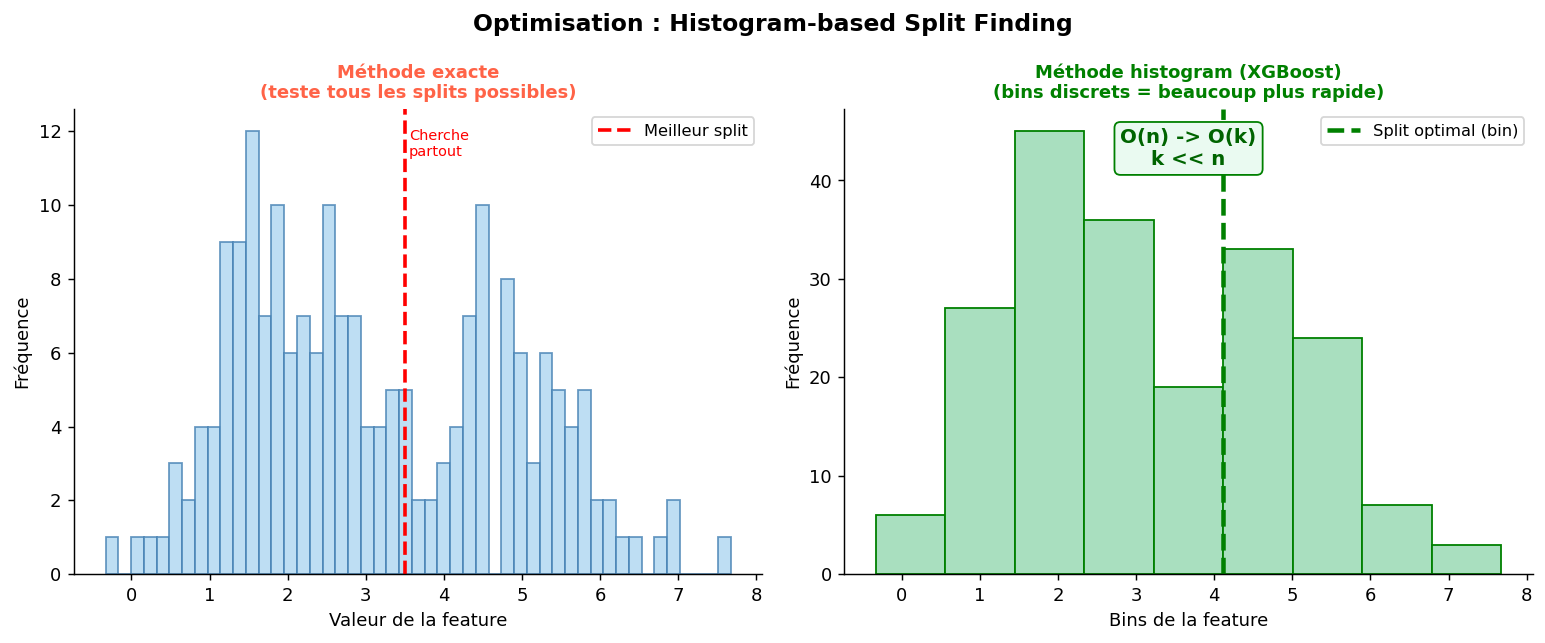
\includegraphics[width=0.95\linewidth]{imagens/xgb_histogram_split.png}
    \caption{XGBoost remplace la recherche exacte par des bins discrets : $O(n) \rightarrow O(k)$ avec $k \ll n$.}
\end{figure}
\end{frame}

% Frame 5 : Apprentissage Parallèle
\begin{frame}{ Apprentissage Parallèle (Column Blocks)}
    \begin{block}{Innovation : Stockage par Blocs de Colonnes}
        \small
        XGBoost stocke les données dans une structure en mémoire appelée \textbf{Block}.
    \end{block}
    
    \scriptsize
    \begin{itemize}
        \item Les données sont pré-triées par colonne avant l'entraînement.
        \item Chaque colonne peut être traitée par un cœur CPU différent \textbf{en parallèle}.
        \item Réduit drastiquement le coût du tri (l'étape la plus lente du boosting).
    \end{itemize}

    \centering
    \resizebox{0.8\textwidth}{!}{
    \begin{tikzpicture}[
        block/.style={rectangle, draw, rounded corners=3pt, thick, align=center, minimum height=1.5cm},
        cpu/.style={rectangle, draw=red!80!black, fill=red!10, thick, rounded corners=2pt, minimum width=2.5cm, minimum height=1.2cm, align=center}
    ]
        % Block Memory
        \node[block, fill=blue!10, draw=blue!80!black, minimum width=2.5cm] (v1) at (0,0) {\textbf{Block 1} \\ \scriptsize Variable A \\ \scriptsize (Triée)};
        \node[block, fill=blue!10, draw=blue!80!black, minimum width=2.5cm] (v2) at (4,0) {\textbf{Block 2} \\ \scriptsize Variable B \\ \scriptsize (Triée)};
        \node[block, fill=blue!10, draw=blue!80!black, minimum width=2.5cm] (v3) at (8,0) {\textbf{Block 3} \\ \scriptsize Variable C \\ \scriptsize (Triée)};
        
        % CPUs
        \node[cpu] (c1) at (0, 2.5) {\textbf{Thread CPU 1} \\ \scriptsize Trouve Split A};
        \node[cpu] (c2) at (4, 2.5) {\textbf{Thread CPU 2} \\ \scriptsize Trouve Split B};
        \node[cpu] (c3) at (8, 2.5) {\textbf{Thread CPU 3} \\ \scriptsize Trouve Split C};
        
        % Arrows
        \draw[<->, thick, -latex] (v1.north) -- (c1.south);
        \draw[<->, thick, -latex] (v2.north) -- (c2.south);
        \draw[<->, thick, -latex] (v3.north) -- (c3.south);
        
        % Parallelism line
        \draw[thick, red, dashed] (-1.5, 1.25) -- (9.5, 1.25) node[right, red!80!black] {\textbf{Recherche en Parallèle}};
    \end{tikzpicture}}
\end{frame}


% Frame 3 : Weighted Quantile Sketch
\begin{frame}{ Esquisse de Quantiles Pondérés}
    \begin{block}{Innovation : Weighted Quantile Sketch}
        \small
        XGBoost ne découpe pas les "buckets" de manière uniforme. Il utilise la \textbf{Hessienne ($h_i$)} comme poids.
    \end{block}
    
    \scriptsize
    \begin{itemize}
        \item Rappel : En classification, $h_i = p_i(1-p_i)$ est la \textbf{confiance} ou la variance.
        \item Les points avec une forte Hessienne (incertitude) méritent des bacs plus précis.
        \item \textbf{Sketch} : Algorithme permettant de trouver ces quantiles sur des données massives avec peu de mémoire.
    \end{itemize}

    \centering
    \resizebox{0.8\textwidth}{!}{
    \begin{tikzpicture}[every node/.style={scale=0.9}]
        % Axe
        \draw[->, thick, -latex] (0,0) -- (10,0) node[right] {Feature $x$};
        
        % Densite de Hessienne
        \draw[thick, blue, fill=blue!10, smooth] (0.5,0) to[out=60, in=180] (2, 0.5) to[out=0, in=180] (4.5, 2.5) to[out=0, in=180] (7, 0.8) to[out=0, in=180] (9,0);
        \node[blue!80!black] at (4.5, 1.8) {\textbf{Distribution des Poids (Hessienne $h_i$)}};
        
        % Decoupage des quantiles proportionnels a l'aire (Hessienne)
        % Zone 1 : faible aire, donc large intervalle x
        \draw[thick, dashed, red] (3.0, 0) -- (3.0, 1.5) node[above] {\tiny Split};
        \draw[<->, thick] (0.5, -0.3) -- (3.0, -0.3) node[midway, below] {$C$};
        
        % Zone 2 : forte aire, intervalle etroit
        \draw[thick, dashed, red] (4.0, 0) -- (4.0, 2.4);
        \draw[<->, thick] (3.0, -0.3) -- (4.0, -0.3) node[midway, below] {$C$};
        
        % Zone 3 : forte aire
        \draw[thick, dashed, red] (5.2, 0) -- (5.2, 2.4);
        \draw[<->, thick] (4.0, -0.3) -- (5.2, -0.3) node[midway, below] {$C$};
        
        % Zone 4 : faible aire, large intervalle
        \draw[thick, dashed, red] (9.0, 0) -- (9.0, 0.0);
        \draw[<->, thick] (5.2, -0.3) -- (9.0, -0.3) node[midway, below] {$C$};
        
        % Commentaire
        \node[red!80!black] at (4.5, -1.0) {\footnotesize Les "buckets" sont plus étroits (plus de splits) là où l'incertitude (la Hessienne) est élevée.};
    \end{tikzpicture}}
\end{frame}

% Frame 4 : Parcimonie (1/3)
\begin{frame}{Parcimonie (1/3) : Valeurs Manquantes}
    \begin{columns}[T]
        \begin{column}{0.45\textwidth}
            \textbf{Réalité des données :}
            \vspace{0.1cm}
            
            \begin{table}
                \centering
                \scriptsize
                \begin{tabular}{|c|c|c|c|}
                    \hline
                    \textbf{ID} & \textbf{Dosage} & \textbf{Effic.} ($y_i$) & \textbf{Résidu} ($r_i$) \\
                    \hline
                    1 & 2 & 0 & -0.5 \\
                    2 & 8 & 1 & +0.5 \\
                    3 & \textbf{NaN} & 1 & +0.5 \\
                    4 & 18 & 0 & -0.5 \\
                    \hline
                \end{tabular}
                \caption{\scriptsize $p_0=0.5 \implies r_i = y_i - 0.5$. Donnée manquante pour l'ID 3.}
            \end{table}
            
            \begin{alertblock}{Le défi}
                \scriptsize
                Les algorithmes classiques rejettent les lignes avec des valeurs manquantes ou nécessitent une imputation ($moyenne$, $médiane$).
            \end{alertblock}
        \end{column}
        
        \begin{column}{0.55\textwidth}
            \begin{block}{L'approche native de XGBoost}
                \small
                XGBoost traite la parcimonie (données vides, zéros, NaN) de manière \textbf{unifiée} et \textbf{apprise}.
                
                \vspace{0.2cm}
                \begin{itemize}
                    \item \textbf{Aucune imputation nécessaire} : On ne "devine" pas la valeur.
                    \item \textbf{Direction par défaut} : On apprend quel chemin (Gauche ou Droit) est le meilleur pour les données manquantes.
                \end{itemize}
            \end{block}
        \end{column}
    \end{columns}
\end{frame}

\begin{frame}{ Parcimonie (2/4) : Test de la Coupure $< 5$}
    \begin{block}{Étape 1 : Tester la coupure valide $< 5$}
        \small
        XGBoost calcule la pertinence de la coupure (Gain) sur les données observées, puis teste l'affectation du \textbf{\textit{NaN}} à Gauche et à Droite.
    \end{block}

    \begin{columns}[T]
        \begin{column}{0.5\textwidth}
            \centering
            \textbf{\scriptsize Scénario A : $NaN$ à GAUCHE}
            \vspace{0.2cm}
            
            \begin{tikzpicture}[
                level 1/.style={sibling distance=2.5cm, level distance=1.2cm},
                every node/.style={circle, draw, align=center, scale=0.6},
                leaf/.style={rectangle, draw, fill=green!10, text width=2cm, scale=0.6}
            ]
                \node {Dosage < 5}
                    child {node[leaf, fill=blue!10] {Valides: 1 \\ \textbf{+ ID 3 (NaN)}}}
                    child {node[leaf, fill=red!10] {Valides: 2, 4}};
            \end{tikzpicture}
            
            \vspace{0.2cm}
            \scriptsize Gain$_A$ = $0.00$
        \end{column}
        
        \begin{column}{0.5\textwidth}
            \centering
            \textbf{\scriptsize Scénario B : $NaN$ à DROITE}
            \vspace{0.2cm}
            
            \begin{tikzpicture}[
                level 1/.style={sibling distance=2.5cm, level distance=1.2cm},
                every node/.style={circle, draw, align=center, scale=0.6},
                leaf/.style={rectangle, draw, fill=green!10, text width=2cm, scale=0.6}
            ]
                \node {Dosage < 5}
                    child {node[leaf] {Valides: 1}}
                    child {node[leaf, fill=blue!10] {Valides: 2, 4 \\ \textbf{+ ID 3 (NaN)}}};
            \end{tikzpicture}
            
            \vspace{0.2cm}
            \scriptsize Gain$_B$ = \textbf{1.33}
        \end{column}
    \end{columns}
\end{frame}

\begin{frame}{ Parcimonie (3/4) : Test de la Coupure $< 13$}
    \begin{block}{Étape 2 : Tester l'autre coupure valide $< 13$}
        \small
        Il répète l'opération pour la coupure suivante (séparant ID 2 et 4).
    \end{block}

    \begin{columns}[T]
        \begin{column}{0.5\textwidth}
            \centering
            \textbf{\scriptsize Scénario C : $NaN$ à GAUCHE}
            \vspace{0.2cm}
            
            \begin{tikzpicture}[
                level 1/.style={sibling distance=2.5cm, level distance=1.2cm},
                every node/.style={circle, draw, align=center, scale=0.6},
                leaf/.style={rectangle, draw, fill=green!10, text width=2cm, scale=0.6}
            ]
                \node {Dosage < 13}
                    child {node[leaf, fill=blue!10] {Valides: 1, 2 \\ \textbf{+ ID 3 (NaN)}}}
                    child {node[leaf, fill=red!10] {Valides: 4}};
            \end{tikzpicture}
            
            \vspace{0.2cm}
            \scriptsize Gain$_C$ = \textbf{1.33}
        \end{column}
        
        \begin{column}{0.5\textwidth}
            \centering
            \textbf{\scriptsize Scénario D : $NaN$ à DROITE}
            \vspace{0.2cm}
            
            \begin{tikzpicture}[
                level 1/.style={sibling distance=2.5cm, level distance=1.2cm},
                every node/.style={circle, draw, align=center, scale=0.6},
                leaf/.style={rectangle, draw, fill=green!10, text width=2cm, scale=0.6}
            ]
                \node {Dosage < 13}
                    child {node[leaf] {Valides: 1, 2}}
                    child {node[leaf, fill=blue!10] {Valides: 4 \\ \textbf{+ ID 3 (NaN)}}};
            \end{tikzpicture}
            
            \vspace{0.2cm}
            \scriptsize Gain$_D$ = $0.00$
        \end{column}
    \end{columns}
\end{frame}

% Frame 6 : Parcimonie (3/3)
\begin{frame}{Parcimonie (4/4) : Arbre Sparsity-Aware Final}
    \begin{columns}[T]
        \begin{column}{0.45\textwidth}
            \textbf{Résultat de l'apprentissage :}
            \vspace{0.3cm}
            
            \begin{itemize}
                \item Le modèle a remarqué que les patients sans donnée de dosage (ID 3) ont souvent une efficacité positive ($y=1$).
                \item La direction par défaut suivra donc le nœud qui mène aux prédictions positives.
            \end{itemize}
        \end{column}
        
        \begin{column}{0.55\textwidth}
            \centering
            \begin{block}{Arbre avec directions par défaut}
                \vspace{0.5cm}
                \begin{tikzpicture}[
                    level 1/.style={sibling distance=4cm, level distance=1.8cm},
                    every node/.style={circle, draw, align=center, scale=0.7},
                    leaf/.style={rectangle, draw, fill=green!10, text width=2.5cm, scale=0.7}
                ]
                \node (root) {Dosage < 13}
                    child {node[leaf] {Feuille G \\ \textcolor{blue}{ID: 1, 2} \textbf{[+3]} \\ $\sum r_{val} = 0.0$ \\ Cover$_{val} = 0.5$}}
                    child {node[leaf, fill=red!10] {Feuille D \\ \textcolor{blue}{ID: 4} \\ $\sum r_{val} = -0.5$ \\ Cover$_{val} = 0.25$}};
                
                % Fleche epaisse pour le defaut
                \draw[->, ultra thick, blue, bend right=30] (root.north) to[out=150, in=90] node[midway, left, scale=0.8, draw=none] {\textbf{Défaut (NaN)}} (-2.5, -1.3);
                \end{tikzpicture}
            \end{block}
            
            \vspace{0.2cm}
            \scriptsize \textit{La flèche bleue indique le chemin automatique \\ pour toute nouvelle donnée manquante.}
        \end{column}
    \end{columns}
\end{frame}


% Frame 6 : Accès Optimisé au Cache
\begin{frame}{ Accès Optimisé au Cache}
    \begin{block}{Cache-Aware Prefetching}
        \small
        Les accès mémoire non contigus ralentissent le CPU. XGBoost utilise un \textbf{Buffer interne}.
    \end{block}
    
    \scriptsize
    \begin{itemize}
        \item Les gradients sont récupérés par blocs pour tenir dans le \textbf{L1/L2 Cache}.
        \item Évite les "Cache Miss" (quand le CPU attend la RAM).
        \item Crucial pour la performance "Extreme" sur processeurs modernes.
    \end{itemize}

    \centering
    \resizebox{0.8\textwidth}{!}{
    \begin{tikzpicture}[
        mem/.style={rectangle, draw=blue!80!black, fill=blue!10, thick, minimum width=2.5cm, minimum height=3cm, rounded corners=2pt, align=center},
        cache/.style={rectangle, draw=orange!80!black, fill=orange!10, thick, minimum width=2.5cm, minimum height=2.5cm, rounded corners=2pt, align=center},
        cpu/.style={rectangle, draw=red!80!black, fill=red!10, thick, minimum width=2.5cm, minimum height=1.5cm, rounded corners=2pt, align=center}
    ]
        % RAM
        \node[mem] (ram) at (0,0) {};
        \node[above] at (ram.north) {\textbf{RAM Principale}};
        \draw[fill=white, draw=gray, thick] (-1.2, -1) rectangle (1.2, 1);
        \node at (0,0) {\scriptsize Gradients};
        \node at (0,-0.5) {\scriptsize non-contigus};
        
        % L1/L2
        \node[cache] (cache) at (5,0) {};
        \node[above] at (cache.north) {\textbf{Cache L1/L2}};
        \draw[fill=white, draw=gray, thick] (3.8, -0.5) rectangle (6.2, 0.5);
        \node at (5,0) {\textbf{Buffer Interne}};
        
        % CPU
        \node[cpu] (cpu) at (10,0) {\textbf{CPU} \\ \scriptsize Calcul Split};
        
        % Connections
        \draw[->, ultra thick, blue, -latex] (ram.east) -- (cache.west) node[midway, above, align=center, scale=0.8] {\textbf{Collecte} \\ par blocs};
        \draw[->, ultra thick, red!80!black, -latex] (cache.east) -- (cpu.west) node[midway, above, align=center, scale=0.8] {\textbf{Accès} \\ immédiat};
        
        % Label
        \node[text=red!80!black, align=center] at (5, -2.2) {\footnotesize Évite au CPU d'attendre la lenteur de la RAM (Cache Miss)};
    \end{tikzpicture}}
\end{frame}

% Frame 7 : Calculs Hors-Mémoire (Out-of-Core)
\begin{frame}{ Calculs Hors-Mémoire (Principe)}
    \begin{block}{Traitement du Big Data}
        \small
        Pour les données plus grandes que la RAM, XGBoost optimise les accès disque.
    \end{block}
    
    \vspace{0.3cm}
    \begin{itemize}
        \item \textbf{Compression par blocs} : Les données sur le disque sont compressées (algorithme LZ4 très performant).
        \item \textbf{Décompression à la volée} : Un thread indépendant du CPU s'occupe de la décompression avant que le modèle n'en ait besoin.
        \item \textbf{Sharding} : Les données sont réparties sur plusieurs disques pour paralléliser les lectures (I/O) et maximiser le débit.
    \end{itemize}
\end{frame}

\begin{frame}{ Calculs Hors-Mémoire (Architecture)}
    \centering
    \vspace{0.5cm}
    \resizebox{0.95\linewidth}{!}{
    \begin{tikzpicture}[
        disk/.style={cylinder, draw=gray!80!black, fill=gray!20, thick, shape border rotate=90, minimum width=2cm, minimum height=2.5cm, align=center},
        block/.style={rectangle, draw=orange!80!black, fill=orange!10, thick, rounded corners=2pt, minimum width=3cm, minimum height=1.5cm, align=center}
    ]
        % Disks
        \node[disk] (d1) at (0, 2.0) {\textbf{Disque 1} \\ \scriptsize Blocs compressés \\ \scriptsize (LZ4)};
        \node[disk] (d2) at (0, -2.0) {\textbf{Disque 2} \\ \scriptsize Blocs compressés \\ \scriptsize (LZ4)};
        
        % Threads deflate
        \node[block] (t1) at (4.5, 2.0) {\textbf{Thread CPU Indépendant} \\ \scriptsize Décompression à la volée};
        \node[block] (t2) at (4.5, -2.0) {\textbf{Thread CPU Indépendant} \\ \scriptsize Décompression à la volée};
        
        % RAM
        \node[rectangle, draw=green!80!black, fill=green!10, thick, rounded corners=2pt, minimum height=6cm, minimum width=3.5cm, align=center] (ram) at (10, 0) {\textbf{RAM Principale} \\ \vspace{0.2cm} \\ \scriptsize Algorithme \\ \scriptsize d'entraînement \\ \scriptsize (XGBoost)};
        
        % Arrows
        \draw[->, ultra thick, gray, -latex] (d1.east) -- (t1.west) node[midway, above] {Lecture};
        \draw[->, ultra thick, gray, -latex] (d2.east) -- (t2.west) node[midway, above, text width=2cm, align=center, yshift=-0.2cm] {Sharding};
        
        \draw[->, ultra thick, blue, -latex] (t1.east) -- (ram.150);
        \draw[->, ultra thick, blue, -latex] (t2.east) -- (ram.210);
    \end{tikzpicture}}
\end{frame}

% ─────────────────────────────────────────────

% ─────────────────────────────────────────────
% IMAGE : Subsampling stochastique
\begin{frame}{Subsampling stochastique — Illustration}
\begin{figure}
    \centering
    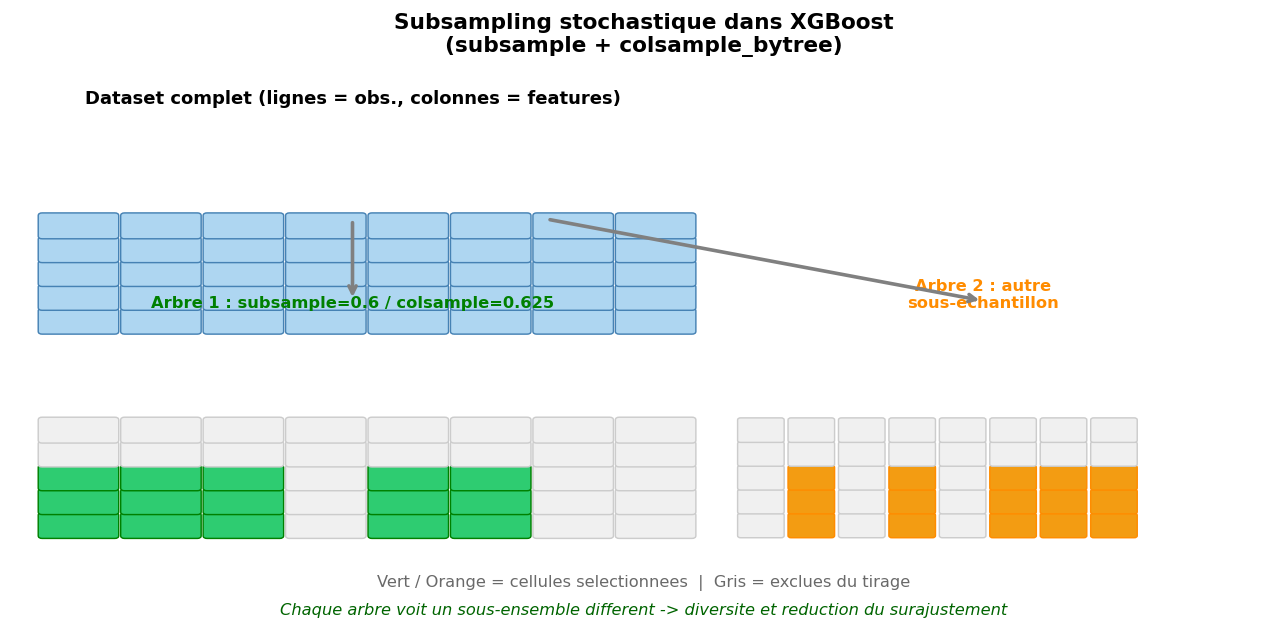
\includegraphics[width=0.92\linewidth]{imagens/xgb_subsampling.png}
    \caption{Chaque arbre reçoit un sous-ensemble différent de lignes et colonnes.}
\end{figure}
\end{frame}

% ─────────────────────────────────────────────
% IMAGE : Early Stopping
\begin{frame}{Early Stopping — Illustration}
\begin{figure}
    \centering
    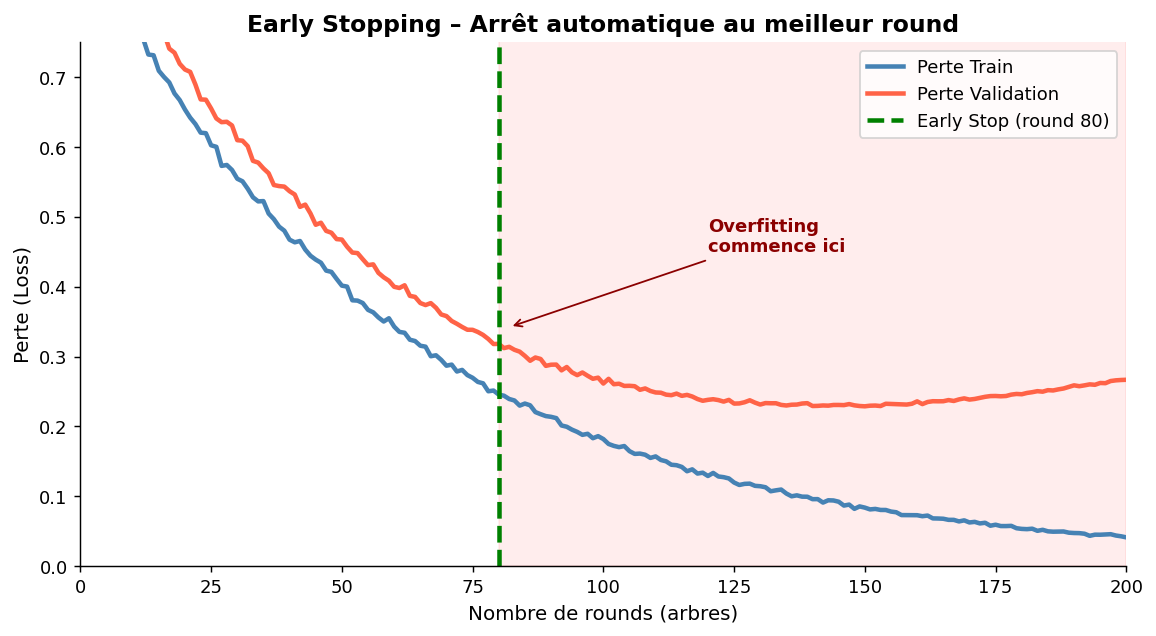
\includegraphics[width=0.90\linewidth]{imagens/xgb_early_stopping.png}
    \caption{L'entraînement s'arrête automatiquement au meilleur round de validation.}
\end{figure}
\end{frame}
\begin{frame}{Régularisation XGBoost — Illustration}
\begin{figure}
    \centering
    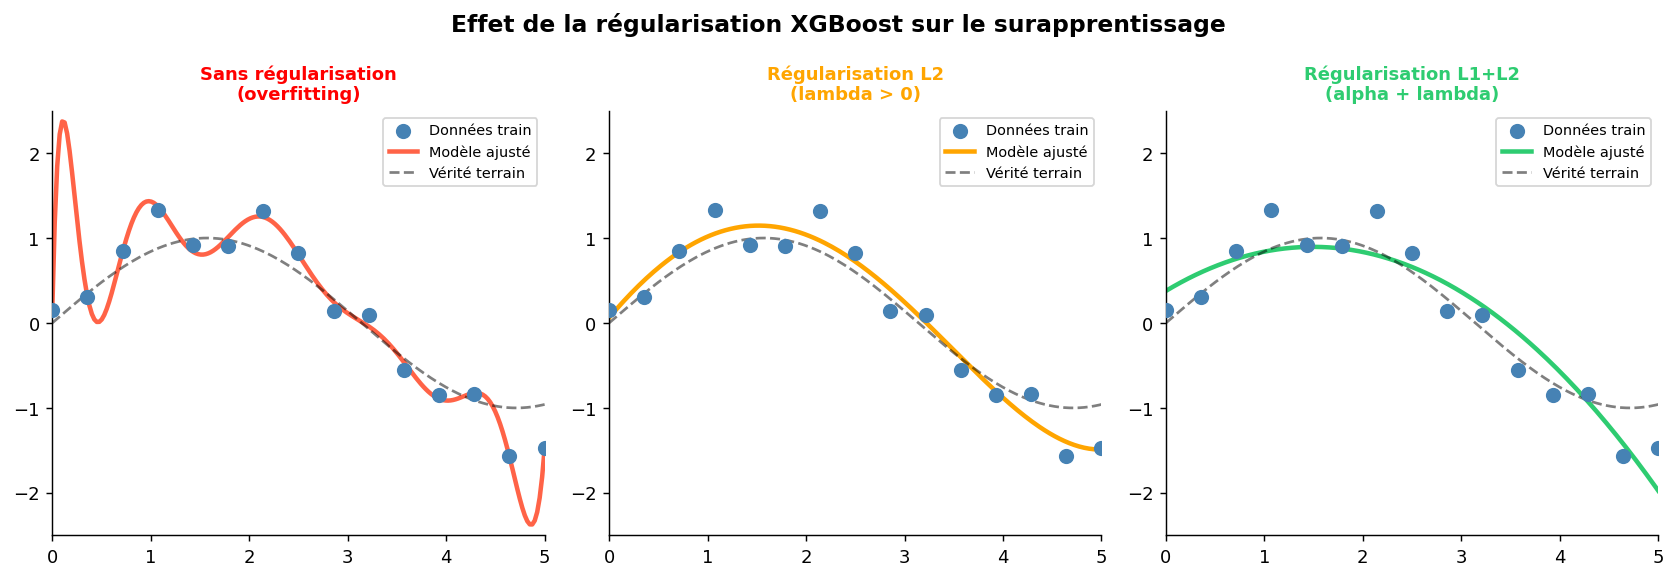
\includegraphics[width=0.97\linewidth]{imagens/xgb_regularization.png}
    \caption{La régularisation L1 (\texttt{alpha}) et L2 (\texttt{lambda}) contrôle le surapprentissage.}
\end{figure}
\end{frame}
% ─────────────────────────────────────────────
\begin{frame}{Limitations du Gradient Boosting classique (GBM)}
\begin{itemize}
    \item Absence de régularisation explicite $\rightarrow$ risque élevé de surapprentissage
    \item Optimisation de premier ordre uniquement (gradient seul)
    \item Gestion limitée des valeurs manquantes
    \item Performances réduites sur grandes bases de données
    \item Manque d'optimisations systèmes pour le passage à l'échelle
\end{itemize}
\end{frame}

% ─────────────────────────────────────────────
% IMAGE : Régularisation L1/L2


% ─────────────────────────────────────────────
\begin{frame}{Optimisations systèmes de XGBoost}
\begin{itemize}
    \item \textbf{Parallélisation} interne : recherche des meilleurs splits en parallèle
    \item Structure en colonnes (\textit{Column Block}) pour accélérer les calculs

    \medskip

    \item Scalabilité sur grandes données :
    \begin{itemize}
        \item \textbf{Histogram-based splits} (discrétisation en bins)
        \item \textbf{Out-of-core computing} (gestion des données hors mémoire)
        \item \textbf{Weighted Quantile Sketch} (approximation efficace des quantiles)
    \end{itemize}
\end{itemize}
\end{frame}

% ─────────────────────────────────────────────

% ─────────────────────────────────────────────
\begin{frame}{Hyperparamètres clés de XGBoost}
\begin{itemize}
    \item \textbf{Contrôle de la complexité :}
    \begin{itemize}
        \item \texttt{max\_depth}, \texttt{min\_child\_weight}, \texttt{gamma}
    \end{itemize}

    \item \textbf{Régularisation et apprentissage :}
    \begin{itemize}
        \item \texttt{lambda} (L2) et \texttt{alpha} (L1)
        \item \texttt{learning\_rate}
    \end{itemize}

    \item \textbf{Sampling et autres :}
    \begin{itemize}
        \item \texttt{subsample}, \texttt{colsample\_bytree}
        \item \texttt{scale\_pos\_weight}
        \item \texttt{n\_estimators} + \texttt{early\_stopping\_rounds}
    \end{itemize}
\end{itemize}
\end{frame}

% ─────────────────────────────────────────────
% IMAGE : Radar chart comparaison
\begin{frame}{Comparaison XGBoost vs Random Forest — Vue Radar}
\begin{figure}
    \centering
    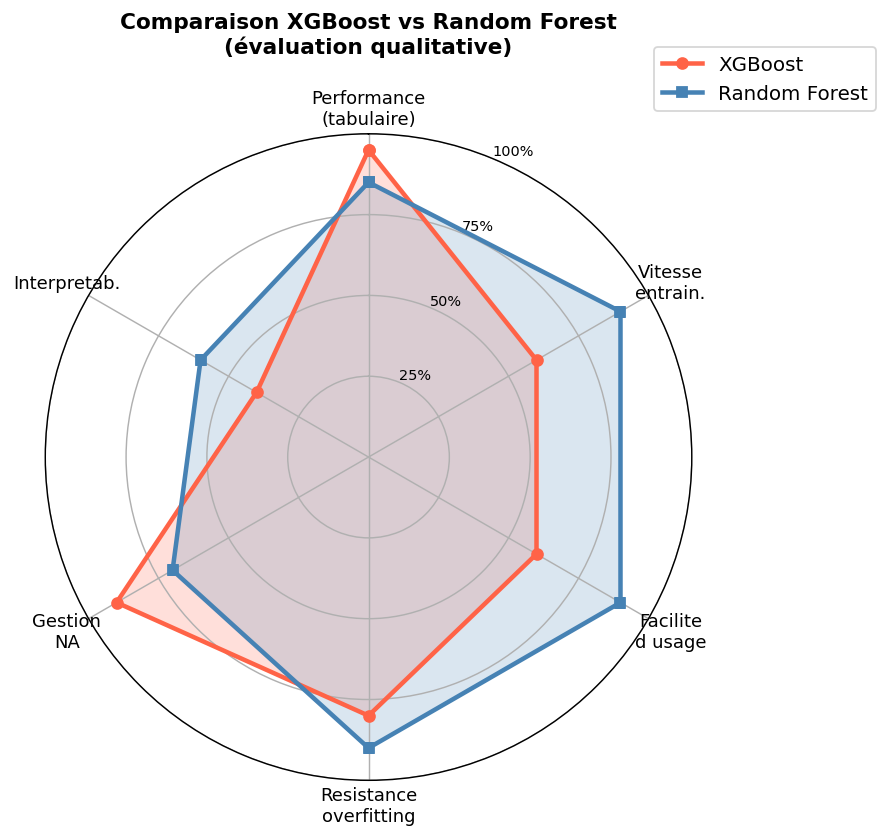
\includegraphics[width=0.68\linewidth]{imagens/xgb_vs_rf_radar.png}
    \caption{Comparaison qualitative sur 6 critères clés.}
\end{figure}
\end{frame}

% ─────────────────────────────────────────────
\begin{frame}{Conclusion XGBoost}
\begin{itemize}
    \item XGBoost représente l'\textbf{état de l'art} du gradient boosting
    \item Trois piliers : \textbf{précision}, \textbf{efficacité} et \textbf{praticité}
    \item Optimisation de second ordre régularisée
    \item Parallélisation et gestion mémoire optimisées
    \item Fonctionnalités natives avancées
    \item Choix privilégié lorsque la \textbf{performance prédictive est critique}

\end{itemize}
\end{frame}


\section{Conclusion Générale}

\begin{frame}{Conclusion Générale}
    \small
    \begin{columns}[T]
    \begin{column}{0.32\textwidth}
        \textbf{SVM}{\small
            \begin{itemize}
                \item Hyperplan à \textbf{marge maximale}
                \item Kernel Trick pour données non linéaires
                \item Optimum \textbf{global} garanti
                \item Sensible aux hyperparamètres ($C$, $\sigma$)
                \item Coûteux sur grands jeux de données
            \end{itemize}}
    \end{column}
    \begin{column}{0.32\textwidth}
        \textbf{Random Forest}{\small
            \begin{itemize}
                \item \textbf{Bagging} d'arbres indépendants
                \item Réduction de la \textbf{variance} via agrégation
                \item Validation intégrée (\textbf{OOB})
                \item Peu sensible aux hyperparamètres
                \item Ne peut pas \textbf{extrapoler}
            \end{itemize}}
    \end{column}
    \begin{column}{0.32\textwidth}
        \textbf{XGBoost}{\small
            \begin{itemize}
                \item \textbf{Boosting} séquentiel régularisé
                \item Approximation de \textbf{Taylor 2\textsuperscript{nd} ordre}
                \item Gestion native des \textbf{valeurs manquantes}
                \item Meilleure performance sur données tabulaires
                \item Réglage plus complexe (+20 hyperparamètres)
            \end{itemize}}
    \end{column}
    \end{columns}
\end{frame}

\begin{frame}{Cas d'étude : Détection du diabète}
    \vspace{5pt}
    \begin{block}{Application : Détection du Diabète (PIDD)}
        \vspace{6pt}
        \begin{columns}[T]
        \begin{column}{0.65\textwidth}
            Les trois algorithmes ont été évalués sur la \textbf{Pima Indians Diabetes Database} (768 patientes, 8 variables cliniques, 35\% de cas positifs).\\[2pt]
            \textbf{XGBoost} obtient les meilleures performances globales (AUC-ROC, F1-score).\\
            \textbf{Random Forest} excelle en robustesse et rappel.\\
            \textbf{SVM (RBF)} est compétitif mais sensible au déséquilibre des classes.
        \end{column}
        \begin{column}{0.32\textwidth}
            \textbf{Variable clé :}\\[2pt]
            La \textbf{glycémie plasmatique} est systématiquement le prédicteur le plus informatif dans les trois modèles.
        \end{column}
        \end{columns}
    \end{block}
\end{frame}

\begin{frame}{The End}
    \centering
    \usebeamerfont{frametitle}{\textbf{\Huge Merci pour votre attention !}}\\[1cm]
    \huge Des questions ?
\end{frame}

\end{document}